\documentclass[12pt]{article}
\usepackage{listings}
\usepackage{enumerate}
\usepackage{xcolor}
\usepackage{graphicx}
\usepackage{booktabs}
\usepackage[italian]{babel}
\usepackage[utf8]{inputenc}
\usepackage{float}
\usepackage{caption}
\usepackage[shortlabels]{enumitem}
\usepackage[T1]{fontenc}
\usepackage{amsfonts}
\usepackage{amsmath}
\usepackage{amssymb}
\usepackage{cancel}
\usepackage[font=small,labelfont=bf]{caption}
\usepackage{dsfont}
\usepackage{enumitem}
\usepackage{fancyhdr}
\usepackage{fancyvrb}
\usepackage{hyperref}
\usepackage{lastpage}
\usepackage{mathtools}
\usepackage{natbib}
\usepackage{parskip}
\usepackage{sectsty}
\usepackage{subfigure}
\usepackage{verbatim}
\usepackage{pgf, tikz}
\usepackage{changepage}

\usetikzlibrary{arrows, automata, positioning, fit,backgrounds}

\definecolor{darkBlue}{rgb}{0.21,0.46,0.80}
\definecolor{notWhite}{HTML}{F2F2EB}
\definecolor{notBlack}{HTML}{272822}
\definecolor{monokai@black}{HTML}{2C2C2A}
\definecolor{monokai@gray}{HTML}{524F52}
\definecolor{monokai@magenta}{HTML}{D33682}
\definecolor{monokai@blue}{HTML}{004C99}
\definecolor{monokai@yellow}{HTML}{FDF5A9}
\definecolor{monokai@orange}{HTML}{FD971F}
\definecolor{monokai@red}{HTML}{DC322F}
\definecolor{monokai@violet}{HTML}{F7208B}
\definecolor{monokai@green}{HTML}{009900}

\lstdefinestyle{R}{
	frame=tb,
	language=R,
	backgroundcolor=\color{notWhite},
	aboveskip=1mm,
	belowskip=1mm,
	showstringspaces=false,
	columns=flexible,
	basicstyle={\small\ttfamily},
	numbers=left,
	numberstyle=\tiny\color{monokai@black},
	numbersep=5pt,
	stepnumber=2,
	breaklines=true,
	tabsize=3,
	numberstyle=\color{monokai@gray},
	keywordstyle=\color{darkBlue},
	stringstyle=\color{monokai@green}\ttfamily,
	identifierstyle=\color{monokai@black},
	commentstyle=\color{monokai@violet},
	emphstyle=\color{monokai@red},
	otherkeywords={0,1,2,3,4,5,6,7,8,9},
    morekeywords={TRUE,FALSE}
}

\newcommand{\redverb}[1]{
	{
	\color{red}
	\verbatiminput{code/#1}
	}
}

\renewcommand{\lstlistingname}{Codice}

\begin{document}
\begin{titlepage}
	\newcommand{\HRule}{\rule{\linewidth}{0.5mm}}

	\center
	
	\textsc{\LARGE Università degli studi di Firenze}\\[1.5cm] 
	
	\textsc{\Large Curriculum Data Science}\\[0.5cm] 
	
	\textsc{\large Inferenza statistica Bayesiana}\\[0.5cm] 

	\HRule\\[0.4cm]
	
	{\huge\bfseries Quaderno degli esercizi}\\[0.4cm] % Title of your document
	
	\HRule\\[1.5cm]
	\vfill\vfill\vfill 

	\begin{minipage}{\textwidth}
		\begin{flushright}
			\large
			\textit{Studente}\\
			\textsc{Filippo Mameli}\\
			\texttt{filippo.mameli@stud.unifi.it}
		\end{flushright}
	\end{minipage}
	
	\vfill
	
	{\large Anno accademico 2017-2018}
	
\end{titlepage}

\newpage

% \tableofcontents

% \newpage

% \thispagestyle{empty}\clearpage\mbox{}\clearpage

\section{Prima Parte}
% \subsection{Esercizio 1 Daboni Wedlin}
Gli eventi $E_{1}, E_{2},  E_{3}, E_{4}, E_{5}$ sono giudicati scambiabili.
Sono assegnate le seguenti probabilità:
\begin{itemize}[label=]
	\item $P(E_{2})=\frac{1}{2}$
	\item $P(E_{3}\wedge E_{5})=\frac{1}{4},$ 
	\item $P(E_{1}\wedge\overline{E}_2\wedge E_{3}\wedge\overline{E}_{4}\wedge E_{5})=P(E_{1}\wedge\overline{E}_{2}\wedge\overline{E}_{3}\wedge\overline{E}_{4}\wedge\overline{E}_{5})=P(E_{1}\wedge E_{2}\wedge E_{3}\wedge E_{4}\wedge E_{5})=\frac{1}{30}$.
\end{itemize}

Si calcolino:
\begin{itemize}[label=]
	\item $P(E_{2}\wedge E_{3}\wedge E_{4})$
	\item $P(E_{1}\wedge E_{2}\wedge E_{3}\wedge E_{4})$
	\item $P(E_{1}\wedge E_{2}\wedge\overline{E}_{3}\wedge\overline{E}_{4}\wedge\overline{E}_{5})$
\end{itemize}

\textbf{Svolgimento}:
\\
\bigskip

Ci troviamo nel caso di un \textit{processo di alternativa semplice limitato} con 5 eventi ($E_{1}, E_{2},  E_{3}, E_{4}, E_{5}$), ai quali corrispondono 5 variabili aleatorie \\
($X_{1}, X_{2},  X_{3}, X_{4}, X_{5}$) sotto l’ipotesi di scambiabilità. Si parla di processo di alternativa semplice limitato poichè gli eventi in questione sono di numero limitato, di tipo elementare (vero-falso) e le variabili indicatrici associate sono di tipo 0-1. \\
L’ipotesi di scambiabilità garantisce che dati \textit{n} eventi, non necessariamente indipendenti, la probabilità che se ne realizzino esattamente \textit{h} su \textit{n} non è dipendente dall'ordine degli eventi stessi ovvero, permutando l’ordine delle variabili indicatrici, la probabilità della loro realizzazione resta immutata. \\

Usando la terminologia dei processi di alternativa semplice indicheremo con:
\begin{itemize}[label=-]
    \item $\omega^n_h$ la probabilità che dati \textit{n} eventi se ne realizzino esattamente \textit{h}, indipendentemente dal loro ordine
     \item $\frac{\omega^n_h}{\binom{n}{h}}$ la probabilità di una singola \textit{traiettoria} formata da una determinata sequenza di \textit{h} successi su \textit{n} prove. Infatti di tali possibili traiettorie ne avremo $\binom{n}{h}$.
    \item $\omega_h$ la probabilità di \textit{h} successi su \textit{h} prove.
\end{itemize}


Possiamo a questo punto riscrivere i dati del nostro problema come segue:
\begin{align*}
	P(E_{2})=\omega_{1}&=\frac{1}{2}\\
	 P(E_{3}\wedge E_{5}) =\omega_{2} &=\frac{1}{4}\\
	 P(E_{1}\wedge\overline{E}_{2}\wedge E_{3}\wedge\overline{E}_{4}\wedge E_{5}) =\frac{\omega_{3}^5}{\binom{5}{3}}&=\frac{1}{30} \\
	 P(E_{1}\wedge\overline{E}_{2}\wedge\overline{E}_{3}\wedge\overline{E}_{4}\wedge\overline{E}_{5}) =\frac{\omega_{1}^5}{\binom{5}{1}}&=\frac{1}{30} \\
	 P(E_{1}\wedge E_{2}\wedge E_{3}\wedge E_{4}\wedge E_{5}) =\omega_{5}&=\frac{1}{30}.
\end{align*}
Ciò che dobbiamo calcolare sarà quindi:
\begin{align*}
 P(E_{2}\wedge E_{3}\wedge E_{4})&=\omega_{3}\\
 P(E_{1}\wedge E_{2}\wedge E_{3}\wedge E_{4})&=\omega_{4}\\
 P(E_{1}\wedge E_{2}\wedge\overline{E}_{3}\wedge\overline{E}_{4}\wedge\overline{E}_{5})&=\frac{\omega_{2}^5}{\binom{5}{2}}
\end{align*}

Dalla teoria dei processi scambiabili sappiamo che le $\omega_h$ e le $\omega^n_h$ sono legate da specifiche relazioni e che è possibile ricavare le une dalle altre. Un modo per ottenere le serie richieste dai dati forniti è quello di sfruttare la seguente equazione:

\begin{align*}
    \omega_h^n = \binom{n}{h}(-1)^{n-h}\cdot\Delta^{n-h}\cdot\omega_h \quad \quad \quad  h\leq n
\end{align*}

Possiamo quindi riscrivere le quantità richieste e date dal problema  in funzione delle $\omega_h$:
\begin{align*}
    \frac{\omega_2^5}{\binom{5}{2}} &= (-1)^3\Delta^3\omega_2=-(\omega_5-3\omega_4+3\omega3-\omega_2)\\
    \frac{\omega_1^5}{\binom{5}{1}} &= (-1)^4\Delta^4\omega_1=\omega_5-4\omega_4+6\omega3-4\omega_2+\omega_1 =  -4\omega_4+6\omega_3-\frac{7}{15} &= \frac{1}{30} \\
    \frac{\omega_3^5}{\binom{5}{3}} &= (-1)^2\Delta^2\omega_3=\omega_5-2\omega_4+\omega_3=-2\omega_4+\omega_3+\frac{1}{30} &= \frac{1}{30} 
\end{align*}

Mettendo a sistema le ultime due equazioni potremo ricavare quanto segue:
\begin{align*}
\begin{cases} 
-4\omega_4+6\omega_3-\frac{7}{15}= \frac{1}{30} \\
-2\omega_4+\omega_3+\frac{1}{30} = \frac{1}{30} 
\end{cases}
\Longrightarrow
\begin{cases} 
\omega_3 = \frac{1}{8}\\
\omega_4 = \frac{1}{16}
\end{cases}\\ \\
\frac{\omega_2^5}{\binom{5}{2}} = -\frac{1}{30}+\frac{3}{16}-\frac{3}{8}+\frac{1}{16} = \frac{7}{240}
\end{align*}

In conclusione, le quantità richieste saranno:
\begin{align*}
	 P(E_2\wedge E_3\wedge E_4) &= \omega_3 = \frac{1}{8}\\
	 P(E_1\wedge E_2\wedge E_3\wedge E_4)&= \omega_4 = \frac{1}{16}\\
	 P(E_1\wedge E_2\wedge\overline{E}_3\wedge\overline{E}_4\wedge\overline{E}_5) &= \frac{\omega_2^5}{\binom{5}{2}} = \frac{7}{240}
\end{align*}


% \newpage
% \subsection{Esercizio 2.6 Hoff}

Conditional independence: Suppose events A and B are conditionally independent given C, which is written $A\perp B|C$. Show that this implies that $A^c\perp B|C$, $A\perp B^c|C$ and $A^c\perp B^c|C$, where $A^c$ means "not A". Find an example where $A\perp B|C$ holds but $A\perp B|C^c$ does not hold.

\textbf{Svolgimento}:
\bigskip

$A\perp B|C$ significa che
$$
	P(A,B|C) = P(A|C)\cdot P(B|C)
$$
Partendo da questa assunzione dobbiamo dimostrare che:
\begin{enumerate}
	\item $P(A^c, B|C) = P(A^c|C)\cdot P(B|C)$
	\item $P(A, B^c|C) = P(A|C)\cdot P(B^c|C)$
	\item $P(A^c, B^c|C) = P(A^c|C)\cdot P(B^c|C)$
\end{enumerate}

Per tutti e 3 i casi partiamo dalla parte destra dell'equazione e dimostriamo che è equivalente alla sinistra, utilizzando l'ipotesi.

\subsubsection{} 
$$
	P(A^c|C)\cdot P(B|C) = (1-P(A|C))\cdot P(B|C) = P(B|C) - P(A|C)\cdot P(B|C) \stackrel{HP}{=} 
$$
$$
	\stackrel{HP}{=} P(B|C) - P(A,B|C) = \frac{P(B,C)}{P(C)} - \frac{P(A,B,C)}{P(C)} = \frac{P(A,B,C^c)}{P(C)} = P(A^c,B|C)
$$

\subsubsection{} 
è analogo al precedente:
$$
	P(A|C)\cdot P(B^c|C) = P(A|C)\cdot (1-P(B|C)) = P(A|C) - P(A|C) \cdot P(B|C)  \stackrel{HP}{=}
$$
$$
	 \stackrel{HP}{=} P(A|C) - P(A,B|C) = \frac{P(A,C)}{P(C)} - \frac{P(A,B,C)}{P(C)} = \frac{P(A,B^c,C)}{P(C)} =P(A,B^c|C)
$$

\subsubsection{}
$$
	P(A^c|C)\cdot P(B^c|C) = (1-P(A|C))\cdot P(1-P(B|C)) =
$$
$$
	= 1 - P(A|C) - P(B|C) + P(A,B|C) \stackrel{HP}{=}
$$
$$
	\stackrel{HP}{=} 1 - P(A|C) - P(B|C) + P(A,B|C) =
$$
$$
	= 1-\frac{P(A,C)}{P(C)} - \frac{P(B,C)}{P(C)} + \frac{P(A,B,C)}{P(C)} = 
$$
$$
	= \frac{P(C)-P(A,C)-P(B,C)+P(A,B,C)}{P(C)} =
$$
$$
 	=\frac{P(A^c,B^c,C)}{P(C)} = P(A^c,B^C|C)
$$
% \newpage
% \subsection{Esercizio 3.7 - Hoff}

Posterior prediction: Consider a pilot study in which $n_1$ = 15 children enrolled in special education classes were randomly selected and tested for a certain type of learning disability. In the pilot study, $y_1$ = 2 children tested positive for the disability.

\begin{enumerate}[label=\alph*)]
    \item Using a uniform prior distribution, find the posterior distribution of $\theta$, the fraction of students in special education classes who have the disability. Find the posterior mean, mode and standard deviation of $\theta$, and plot the posterior density.
    \par Researchers would like to recruit students with the disability to participate in a long-term study, but first they need to make sure they can recruit enough students. Let $n_2 = 278$ be the number of children in special education classes in this particular school disctrict, and let $Y_2$ be the number of students with the disability.
    
    \item find $Pr(Y_2=y_2 | Y_1 = 2)$, the posterior predictive disctribution of $Y_2$, as follows:
    \begin{enumerate}[label=\roman*.]
        \item Discuss what assumptions are needed about the joint distribution of $(Y_1,Y_2)$ such that the following is true:
        \begin{align*}
            Pr(Y_2=y_2) = \int_0^1 Pr(Y_2=y_2|\theta)p(\theta|Y_1=2)\ d\theta 
        \end{align*}
        \item Now plug in the forms for $Pr(Y_2=y_2|\theta)$ and $p(\theta|Y_1=2)$ in the above integral.
        \item Figure out what the above integral must be by using the calculus result discussed in Section 3.1
    \end{enumerate}
    \item Plot the function $Pr(Y_2=y_2|Y_1=2)$ as a function of $y_2$. Obtain the mean and standard deviation of $Y_2$, given $Y_1$=2.
    \item The posterior mode and the MLE (maximum likelihood estimate; see Excercise 3.14) of $\theta$, based on data from the pilot study, are both $\hat{\theta} = 2/15$. Plot the distribution $Pr(Y_2=y_2|\theta=\hat{\theta})$, and find the mean and standard deviation of $Y_2$ give $\theta=\hat{\theta}$. Compare these results to the plots and calculations in c) and discuss any differences. Which distribution for $Y_2$ would you use to make prediction, and why?
\end{enumerate}

\textbf{Svolgimento}
\bigskip

a) Possiamo modellare lo studio trattato nel testo con una distribuzione binomiale ovvero

\begin{align*}
    P(\textbf{y}|\theta) = \theta^{y}(1-\theta)^{1-y}
\end{align*}

e come indicato dal testo useremo come prior una uniforme

\begin{align*}
    P(\theta)= \mathds{1}[0,1]^\theta
\end{align*}

Procediamo adesso al calcolo della \textit{a posteriori}.

\begin{align*}
    P(\theta|\textbf{y}) &= K  \times \mathcal{L}(\theta;\textbf{y})\times P(\theta)\\
    &= K \times \left(\prod_{i=1}^{15}\theta^{y_i}(1-\theta)^{1-y_i}\right)\times\mathds{1}[0,1]^\theta\\
    &\text{...avendo 2 ``successi'' e 13 ``insuccessi'' avremo...} \\
    &= K \times \theta^2(1-\theta)^{13} \times \mathds{1}[0,1]^\theta
\end{align*}

Per calcolare il valore $K$ e volendo trovare una distribuzione di probabilità propria, sappiamo che l'integrale di quest'ultima dovrà essere uguale a 1 nello spazio ammissibile di $\theta$, ovvero

\begin{align*}
   1 &= \int_0^1 K \times \theta^2(1-\theta)^{13} \times \mathds{1}[0,1]^\theta\ d\theta \\
    &= K \int_0^1  \theta^2(1-\theta)^{13}\ d\theta
\end{align*}

Si riconosce il kernel di una distribuzione Beta(3,14) e quindi si può moltiplicare e dividere per la sua costante di normalizzazione
\begin{align*}
    1 &= K \int_0^1  \theta^2(1-\theta)^{13} \frac{\Gamma(17)}{\Gamma(3)\Gamma(14)} \frac{\Gamma(3)\Gamma(14)}{\Gamma(17)}\ d\theta\\
    &= K \times \frac{\Gamma(3)\Gamma(14)}{\Gamma(17)} \underbrace{\int_0^1  \theta^2(1-\theta)^{13} \frac{\Gamma(17)}{\Gamma(3)\Gamma(14)}\ d\theta}_\text{=1}\\
    \frac{1}{K}&=\frac{\Gamma(3)\Gamma(14)}{\Gamma(17)}
\end{align*}

Si conclude quindi che

\begin{align*}
    P(\theta|\textbf{y}) &= \frac{\Gamma(17)}{\Gamma(3)\Gamma(14)} \theta^2(1-\theta)^{13} \\
    &\sim Beta(3,14)
\end{align*}

dalla quale si può facilmente calcolare valore medio, moda e standard deviation

\begin{align*}
    E(\theta|\textbf{y}) &= \frac{\alpha}{\alpha + \beta} = \frac{3}{17}\\
    Moda(\theta|\textbf{y}) &= \frac{\alpha-1}{\alpha + \beta-2} = \frac{2}{15}\\
    Var(\theta|\textbf{y}) &= \frac{\alpha\beta}{(\alpha + \beta)^2(\alpha + \beta + 1)} = \frac{42}{17^2\times 18} \approx 8*10^{-3}
\end{align*}

In Figura \ref{fig:beta} si mostra la distribuzione appena calcolata

\begin{figure}[!ht]
\centering
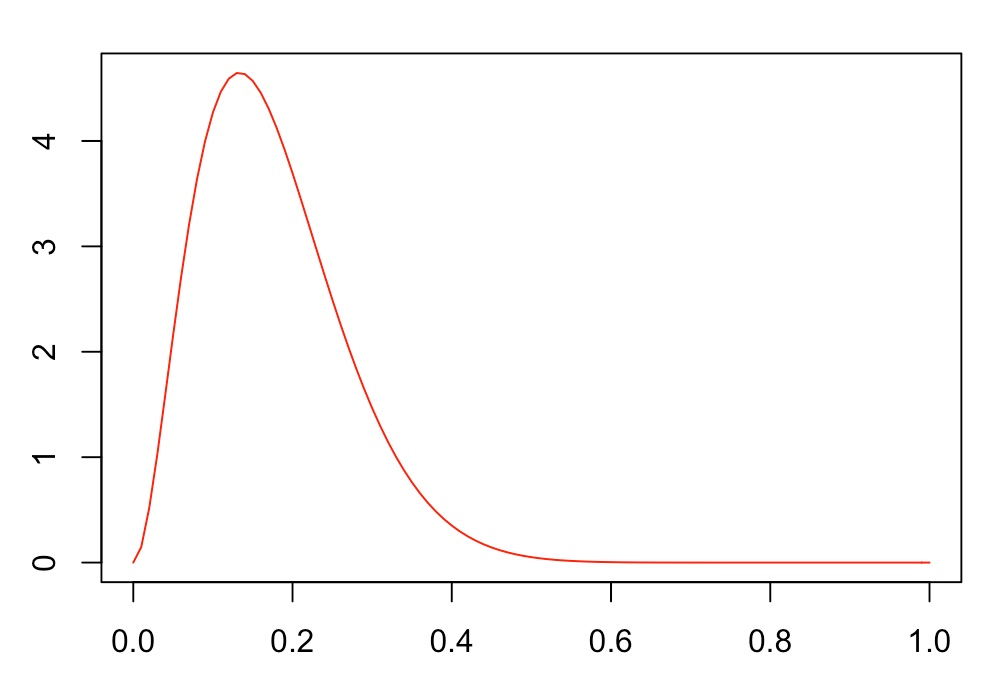
\includegraphics[width=0.6\textwidth]{img/esercizio3-07-Beta314}
\caption{una Beta(3,14)}
\label{fig:beta}
\end{figure}

b) Affinchè
\begin{equation} \label{eq:1}
    Pr(Y_2=y_2) = \int_0^1 Pr(Y_2=y_2|\theta)p(\theta|Y_1=2) \ d\theta
\end{equation}
dobbiamo innanzitutto assumere che la distribuzione predittiva non dipenda da quantità 
incognite ma dipenda dai dati osservati (altrimenti sarebbe inutilizzabile ai fini 
predittivi), ma che il valore predetto sia indipendente dai dati osservati dato $\theta$, ovvero 
\begin{align*}
    Y_2 \perp\!\!\!\perp Y_1 | \theta \\
    (\text{ma non } Y_2 \perp\!\!\!\perp Y_1)
\end{align*}

Con queste assunzioni otterremo che $Pr(Y_2|\theta,Y_1) = Pr(Y_2|\theta)$ e quindi l'equazione (\ref{eq:1}) risulterà valida. \\
Considerando le assunzioni del testo e svolgendo i calcoli avremo quanto segue:

\begin{align*}
     Pr(Y_2=y_2) &= \int_0^1 Pr(Y_2=y_2|\theta)p(\theta|Y_1=2) \ d\theta\\
     &= \int_0^1 \binom{278}{y_2}\theta^{y_2}(1-\theta)^{278-y_2} \frac{\Gamma(17)}{\Gamma(3)\Gamma(14)} \theta^2(1-\theta)^{13}\ d\theta\\
      &= \binom{278}{y_2} \frac{\Gamma(17)}{\Gamma(3)\Gamma(14)} \int_0^1 \theta^{y_2 + 2}(1-\theta)^{291-y_2}\ d\theta
\end{align*}

Si riconosce nell'integrale il kernel di una Beta($y_2+3,292-y_2$) e quindi utilizzando 
la stessa tecnica vista al punto precedente avremo

\begin{align*}
     Pr(Y_2=y_2) &= \binom{278}{y_2} \frac{\Gamma(17)}{\Gamma(3)\Gamma(14)} \frac{\Gamma(y_2+3)\Gamma(292-y_2)}{\Gamma(295)}\\
     &=  \frac{\Gamma(3+14)}{\Gamma(3)\Gamma(14)\Gamma(3+14+278)}\binom{278}{y_2} \Gamma(3+y_2)\Gamma(14+278-y_2)
\end{align*}

ovvero una \textbf{Beta-Binomiale(3, 14, 278)} 
(rappresentata in Figura \ref{fig:betaBinomiale}) dalla quale si può 
facilmente calcolare media e standard deviation:

\begin{align*}
    E(Y_2|Y_1=2) &= n\frac{\alpha}{\alpha + \beta} = 278\frac{3}{17} \approx 49,06\\
    Var(Y_2|Y_1=2) &= \frac{n\alpha\beta}{(\alpha + \beta)^2}\times\frac{(\alpha + \beta + n)}{(\alpha + \beta + 1)} = \frac{278\times3\times14}{17^2} \times\frac{295}{18} \approx 662,13
\end{align*}


\begin{figure}[!ht]
\centering
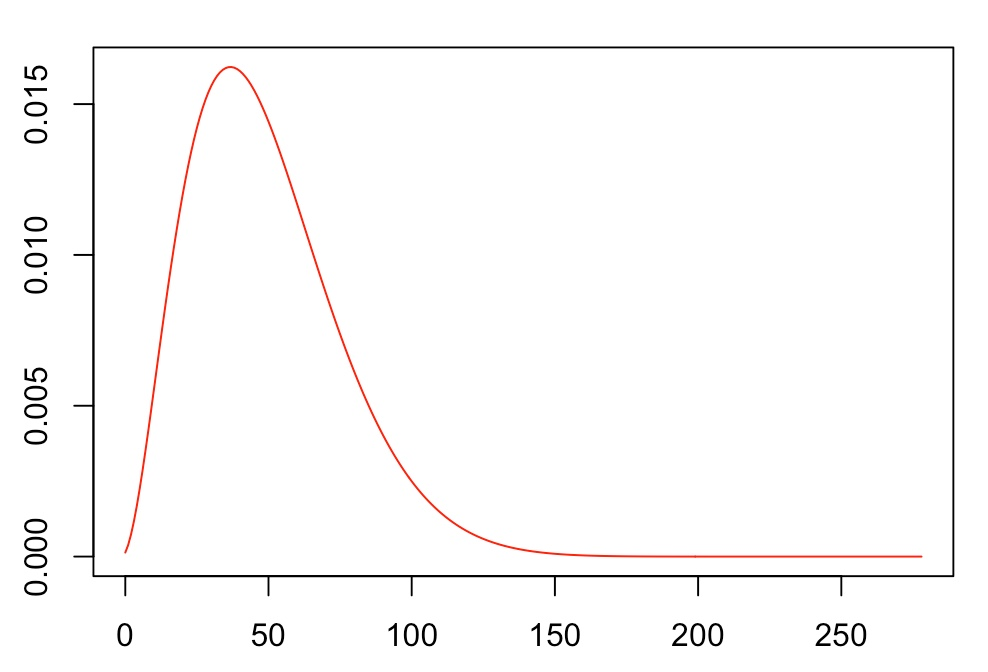
\includegraphics[width=0.6\textwidth]{img/esercizio3-07-BetaBinomiale}
\caption{Beta-Binomiale(3, 14, 278)}
\label{fig:betaBinomiale}
\end{figure}

Supponendo che la moda a posteriori e la MLE di $\theta$ siano entrambe $\hat{\theta}$ = 2/15 allora avremo 

\begin{align*}
    P\left(Y_2=y_2|\theta=\frac{2}{15}\right) &= \binom{278}{y_2}\left(\frac{2}{15}\right)^{y_2}\left(1-\frac{2}{15}\right)^{278-y_2} \\
    &\sim Binomiale\left(\frac{2}{15},278\right)
\end{align*}

Otteniamo quindi una distribuzione binomiale (rappresentata nella parte destra di Figura \ref{fig:Binomiale}) con relative media e standard deviation:

\begin{align*}
    E\left(Y_2=y_2|\theta=\frac{2}{15}\right) &= n\theta = 278\times\frac{2}{15} \approx 37,07\\
    Var\left(Y_2=y_2|\theta=\frac{2}{15}\right)  &= n\theta (1-\theta) = 278\times\frac{2}{15} \times \frac{13}{15} \approx 32,12
\end{align*}


\begin{figure}[!ht]
\begin{minipage}[b]{0.47\textwidth}
\centering
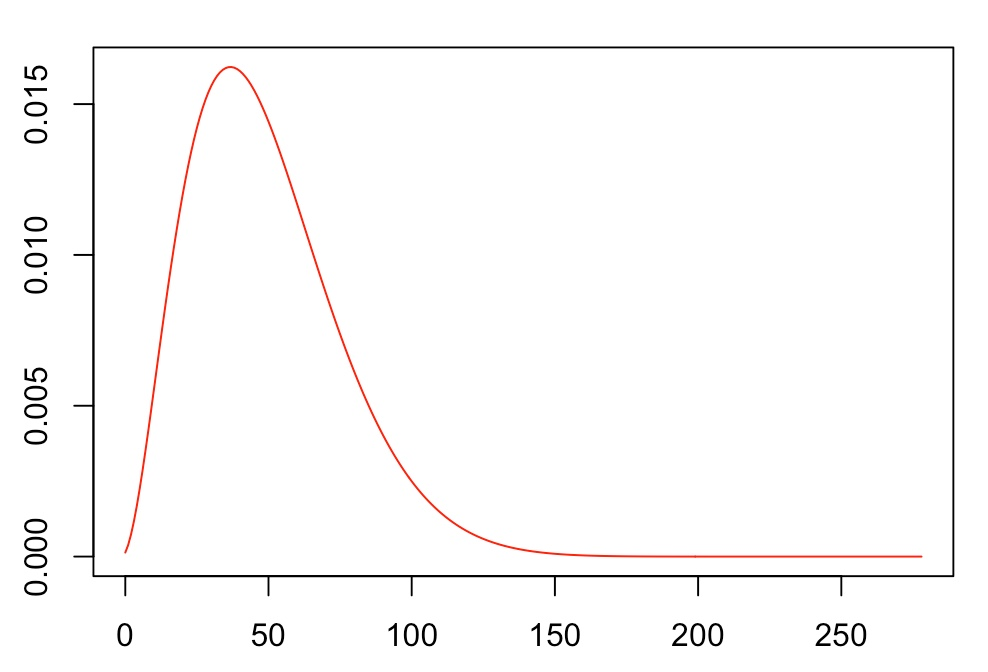
\includegraphics[width=\textwidth]{img/esercizio3-07-BetaBinomiale}
\end{minipage}
\hfill
\begin{minipage}[b]{0.47\textwidth}
\centering
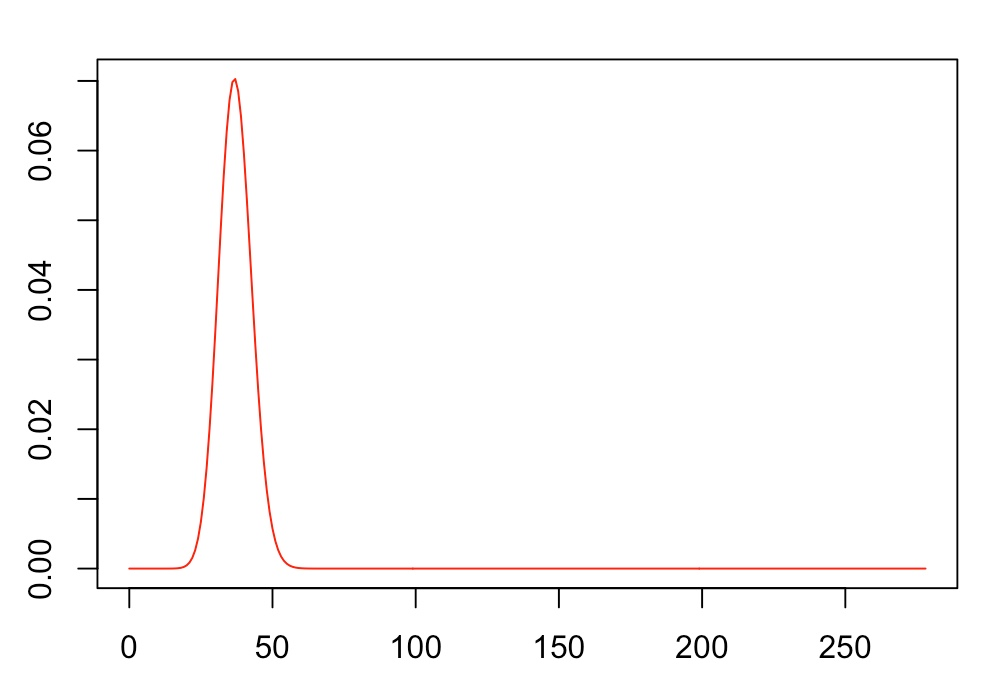
\includegraphics[width=\textwidth]{img/esercizio3-07-Binomiale}
\end{minipage}
\caption{Una Betabinomiale(3, 14, 278) (a sinistra) e una Binomiale(2/15, 278) (a destra) a confronto}.
\label{fig:Binomiale}
\end{figure}

Risulta evidente come media e moda delle due distribuzioni siano piuttosto simili a 
differenza della varianza che risulta notevolmente più bassa nella Binomiale. 
Questo risultato piuttosto intuitivo è dovuto all'aver fissato il parametro $\theta$ 
nel secondo metodo, che ha come effetto una drastica riduzione dell'intervallo di 
confidenza rispetto alla media della nostra predizione. 

Concludendo, per la  predizione di $Y_2$, preferiremo utilizzare quest'ultima variante 
ovvero assegnare a $\theta$ la MLE, che nonostante sia in leggera contrad\-dizione con 
la definizione bayesiana di \textit{a priori} (come vedremo nell'esercizio 3.14) ha 
come effetto una notevole riduzione della variabilità della nostra predizione.
% \newpage
% \subsection{Esercizio 3.14 - Hoff}

Unit information prior: Let $Y_1,...,Y_n \sim $ i.i.d.$p(y|\theta)$. Having
observed the values $Y_1=y_1,...,Y_n=y_n$, the \textit{log likelihood} is given
by $l(\theta|\textbf{y})=\sum\log p(y_{i}|\theta)$, and the value $\hat{\theta}$ of
$\theta$ that maximizes $l(\theta|\textbf{y})$ is called the \textit{maximum
likelihood estimator}. The negative of the curvature of the loglikelihood,
$J(\theta)=-\frac{\partial^{2}l(\theta| \textbf{y})}{\partial\theta^{2}}$, describes
the precision of the MLE $\hat{\theta}$ and is called the \textit{observed
Fisher information}. For situations in which it is difficult to quantify
prior information in terms of a probability distribution, some have
suggested that the \textquotedblleft prior\textquotedblright{} distribution
be based on the likelihood, for example, by centering the prior distribution
around the MLE $\hat{\theta}$. To deal with the fact that the MLE
is not really prior information, the curvature of the prior is chosen
so that it has only \textquotedblleft one \textit{n}th\textquotedblright{}
as much information as the likelihood, so that $-\frac{\partial^{2}\log p(\theta)}{\partial\theta^{2}}=\frac{J(\theta)}{n}$. Such
a prior is called a \textit{unit information prior} (Kass and Wasserman, 1995;
Kass and Raftery, 1995), as it has as much information
as the average amount of information from a single observation. The
unit information prior is not really a prior distribution, as it is
computed from the observed data. However, it can be roughly viewed
as the prior information of someone with weak but accurate prior information. 

\begin{enumerate}[label=\alph*)]
\item Let $Y_1, . . . , Y_n \sim $ i.i.d. binary($\theta$). Obtain the MLE $\hat{\theta}$
and J($\hat{\theta}$)/n.

\item Find a probability density $p_U(\theta)$ such that $\log p_U(\theta) = \frac{l(\theta| \textbf{y})}{n}+c$, where $c$ is a constant that does not depend on $\theta$. Compute the information $-\frac{\partial^{2}\log p(\theta)}{\partial\theta^{2}}$ of this density. 

\item Obtain a probability density for $\theta$ that is proportional to $p_U(\theta) \times p(y_1,\cdots,y_n|\theta)$. Can this be considered a posterior distribution for $\theta$?

\item Repeat a), b) and c) but with $p(y|\theta)$ being the Poisson distribution.

\end{enumerate}

\textbf{Svolgimento}
\\
\bigskip

a) Nel caso analizzato la funzione di densità sarà una Bernuoulli:
\begin{center}
$p(y|\theta)=\theta^{y}(1-\theta)^{1-y}$
\end{center}

e la relativa funzione di verosimigliana per un campione di n osservazioni i.i.d. sarà 
\begin{align*}
\mathcal{L}(\theta: \textbf{y})=\prod_{i=1}^n\theta^{y_i}(1-\theta)^{1-y_i}
\end{align*}

Calcolandonde il logaritmo otterremo la funzione di log-verosomiglianza seguente
\begin{align*}
l(\theta:\textbf{y})=\left(\sum_{i=1}^n y_{i}\right)ln(\theta)+\left(n-\sum_{i=1}^n y_{i}\right)ln(1-\theta)
\end{align*}

Calcoliamo adesso lo stimatore di massima verosomiglianza per $\theta$ che indicheremo con $\hat{\theta}$, ottenuto ponendo a zero la derivata prima della log-verosomiglianza, ovvero
\begin{align*}
\frac{\partial l(\theta;\textbf{y})}{\partial\theta}&=\frac{\sum_{i=1}^{n}y_i}{\theta}-\frac{n-\sum_{i=1}^{n}y_i}{1-\theta}= 0\\
&= \frac{\sum_{i=1}^{n}y_i -
\cancel{\theta\sum_{i=1}^{n}y_i} -
n\theta +
\cancel{\theta\sum_{i=1}^{n}y_i}}
{\theta(1-\theta)} = 0 \\
&=\frac{\sum_{i=1}^{n}y_i}{n} = \hat{\theta} = MLE
\end{align*}

Adesso dobbiamo calcolarci l'informazione osservata di Fisher, ovvero $J(\hat{\theta}) = -\frac{\partial^2 l(\theta;\textbf{y})}{\partial\theta^2}$, dove al posto di $\theta$ sostituiamo $\hat{\theta}$ per ottenere una misura dell'informazione nel punto di massima verosomiglianza.
\begin{align*}
\frac{\partial^2 l(\theta;\textbf{y})}{\partial\theta^2} &= -\frac{\sum_{i=1}^{n}y_i}{\theta^2}+\frac{n-\sum_{i=1}^{n}y_i}{(1-\theta)^2}\\
J(\theta) = -\frac{\partial^2 l(\theta;\textbf{y})}{\partial\theta^2} &= \frac{\sum_{i=1}^{n}y_i}{\theta^2}-\frac{n-\sum_{i=1}^{n}y_i}{(1-\theta)^2}
\end{align*}

e sostituendo $\theta$ col nostro stimatore di massima verosomiglianza $\hat{\theta}$ avremo
\begin{align*}
J(\hat{\theta}) = n\left(\frac{\hat{\theta}}{\hat{\theta^2}} - 
\frac{1- \hat{\theta}}{(1- \hat{\theta})^2}\right)
= n\left(\frac{1}{\hat{\theta^2}} -
\frac{ 1 }{1- \hat{\theta}}\right)
\end{align*}

L'esercizio chiede di calcolare $\frac{J(\hat{\theta})}{n}$ ovvero l'informazione associata alla unit information prior. Otteremo quindi

\begin{align*}
\frac{J(\hat{\theta})}{n} = \left(\frac{1}{\hat{\theta^2}} -
\frac{ 1 }{1- \hat{\theta}}\right)
\end{align*}

\bigskip
b) L'esercizio richiede che
\begin{align*}
\log p_U(\theta) = \frac{l(\theta|y)}{n}+c
\end{align*}

ovvero 
\begin{align*}
\log p_U(\theta)  = \frac{\left(\sum_{i=1}^n y_i\right)ln(\theta)}{n}+\frac{\left(n-\sum_{i=1}^n y_i\right)ln(1-\theta)}{n}
\end{align*}

e riportandosi all'esponente della formula appena scritta otteremo la unit information prior:

\begin{align*}
p_U(\theta)  &= \theta^\frac{\sum_{i=1}^n y_i}{n} 
(1-\theta)^{1-\frac{\sum_{i=1}^n y_i}{n}} 
e^c\\
&\sim Beta(\hat{\theta} + 1, 2 - \hat{\theta})
\end{align*}

A questo punto per calcolare l'informazione di Fisher come richiesto dall'esercizio dobbiamo come primo passo calcolare la derivata prima:

\begin{align*}
\frac{\partial p_U(\theta)}{\partial\theta} &= \frac{\sum_{i=1}^{n}y_i}{n\theta}-
\frac{n-\sum_{i=1}^{n}y_i}{n(1-\theta)}
\end{align*}

Poi la derivata seconda:

\begin{align*}
\frac{\partial^2 p_U(\theta)}{\partial\theta^2} &= -\frac{\sum_{i=1}^{n}y_i}{n\theta^2}+
\frac{n-\sum_{i=1}^{n}y_i}{n(1-\theta)^2}
\end{align*}

Cambiando di segno alla derivata seconda otteremo l'informazione di Fisher:

\begin{align*}
J_U(\theta) = -\frac{\partial^2 p_U(\theta)}{\partial\theta^2} &= \frac{\sum_{i=1}^{n}y_i}{n\theta^2} -
\frac{n-\sum_{i=1}^{n}y_i}{n(1-\theta)^2} = \frac{J(\theta)}{n}
\end{align*}

Notiamo che l'informazione di Fisher per la unit information prior $J_U(\theta)$ non è altro che un \textit{n}-esimo dell'informazione di Fisher per l'intero campione $J(\theta)$, quindi la distribuzione ottenuta rispetta la proprietà desiderata.

\bigskip
c)  L'esercizio chiede di trovare una densità di probabilità per $\theta$ che sia proporzionale a $p_U(\theta) \times p(y_1,\cdots,y_n|\theta)$. Procediamo quindi a svolgere i calcoli richiesti nell'intento di riconoscere il kernel di una distribuzione nota:

\begin{align*}
p_U(\theta) \times \mathcal{L}(\theta;\textbf{y}) &\propto
\theta^\frac{\sum_{i=1}^n y_i}{n} 
(1-\theta)^{1-\frac{\sum_{i=1}^n y_i}{n}} 
\theta^ {\sum_{i=1}^n y_i}
(1-\theta)^{n-\sum_{i=1}^n y_i}\\
&\propto \theta^{\sum_{i=1}^n y_i(1+\frac{1}{n}) }
(1-\theta)^{(n+1) - \sum_{i=1}^n y_i (1+\frac{1}{n}) }
\end{align*}

Riconosciamo il kernel di una Beta, ovvero:


\begin{align*}
p_U(\theta) \times \mathcal{L}(\theta;\textbf{y}) &\propto 
Beta
\left( 
\sum_{i=1}^n y_i\left(1+\frac{1}{n}\right)  + 1, 
(n+2) - \sum_{i=1}^n y_i \left(1+\frac{1}{n}\right) 
\right)
\end{align*}

Se avessimo lavorato con una a priori classica potremmo  concludere che:

\begin{align*}
p_U(\theta|\textbf{y}) =
Beta
\left( 
\sum_{i=1}^n y_i\left(1+\frac{1}{n}\right)  + 1, 
(n+2) - \sum_{i=1}^n y_i \left(1+\frac{1}{n}\right) 
\right)
\end{align*}

ma nel nostro caso non abbiamo usato una vera e propria \textit{a priori}, bensì una \textit{unit information prior} che per sua definizione viene ricavata dal campione e non da una pregressa conoscenza del fenomeno analizzato come impone la definizione di ``a priori" della statistica bayesiana. Possiamo però interpretare questa unit information prior, come l’informazione a priori di una persona che è riuscita a centrare la sua distribuzione sullo stimatore di massima verosimiglianza, ma che è molto insicuro di questa sua informazione (per questo dividiamo l’informazione di Fisher per n in modo da aumentarne la varianza). Solo se applichiamo questo ragionamento possiamo considerare la distribuzione trovata come una a posteriori.

\bigskip
d) Ripetiamo l'intero esercizio ma considerando $p(y|\theta)$ come una distribuzione di Poisson, ovvero:

\begin{align*}
p(y|\theta) = \frac{e^{-\theta}\theta^y}{y!}
\end{align*}

La relativa verosomiglianza per un campione i.i.d. sarà

\begin{align*}
p(y|\theta) = \prod_{i=1}^n \frac{e^{-\theta}\theta^{y_i}}{y_i!}
\end{align*}

e la log-likelihood

\begin{align*}
l(\theta;\textbf{y}) = -n\theta + \left(\sum_{i=1}^n y_i \right)ln(\theta)-ln\prod_{i=1}^n y_i!.
\end{align*}

Calcoliamo come fatto in precedenza lo stimatore di massima verosomiglianza $\hat{\theta}$:

\begin{align*}
\frac{\partial l(\theta; \textbf{y})}{\partial\theta} = -n + \frac{\sum_{i=1}^n y_i}{\theta}
\end{align*}

Ponendola uguale a zero avremo:

\begin{align*}
 -n + \frac{\sum_{i=1}^n y_i}{\theta} &= 0\\
 \frac{\sum_{i=1}^n y_i}{\theta} &= \hat{\theta} = MLE
\end{align*}

Procediamo adesso al calcolo dell'informazione osservata di FIsher $J(\hat{\theta})$ e quindi alla derivata seconda:

\begin{align*}
\frac{\partial^2 l(\theta; \textbf{y})}{\partial\theta^2} = - \frac{\sum_{i=1}^n y_i}{\theta^2}
\end{align*}

Sostituendo a $\theta$ lo stimatore di massima verosomiglianza $\hat{\theta}$ avremo l'informazione osservata:


\begin{align*}
J(\hat{\theta}) = \frac{n}{\hat{\theta}}
\end{align*}

L'esercizio chiede di calcolare $\frac{J(\hat{\theta})}{n}$ ovvero un \textit{n}-esimo dell'informazione osservata di Fisher relativa al campione, che corrisponde all'informazione associata alla unit information prior:

\begin{align*}
\frac{J(\hat{\theta})}{n} = \frac{1}{\hat{\theta}}
\end{align*}

Calcoliamo adesso come chiesto 

\begin{align*}
\log p_U(\theta) &= \frac{l(\theta|y)}{n}+c\\
 &= -\theta + \frac{\sum_{i=1}^n y_i}{n} ln(\theta) \underbrace{ -\frac{ln(\prod_{i=1}^n y_i)}{n} + c }_\text{$c^*$}
\end{align*}

Riportandosi all'esponente avremo:
\begin{align*}
p_U(\theta) &= e^{-\theta}\theta^{\frac{\sum_{i=1}^n y_i}{n}}e^{c^*}\\
&\sim Gamma(\hat{\theta}+1,1)
\end{align*}

Per calcolare l'informazione di Fisher dobbiamo calcolare come primo passo la derivata prima:

\begin{align*}
\frac{\partial p_U(\theta)}{\partial\theta} = -1 + \frac{\sum_{i=1}^n y_i}{n\theta}
\end{align*}

Di conseguenza, la derivata seconda sara:

\begin{align*}
\frac{\partial^2 p_U(\theta)}{\partial\theta^2} = - \frac{\sum_{i=1}^n y_i}{n\theta^2}
\end{align*}

Possiamo adesso calcolare la unit information prior come richiesto

\begin{align*}
J_U(\theta)= - \frac{\partial^2 p_U(\theta)}{\partial\theta^2} = \frac{\sum_{i=1}^n y_i}{n\theta^2} = \frac{J(\theta)}{n}
\end{align*}

Procedendo adesso ad indentificare una distribuzione di densità nota per $  p_U(\theta) \times \mathcal{L}(\theta;\textbf{y}) $ avremo 

\begin{align*}
p_U(\theta) \times \mathcal{L}(\theta;\textbf{y}) &\propto e^{-\theta} \theta  ^ {\frac{\sum_{i=1}^n y_i}{n}} e^{-n\theta}\theta^{\sum_{i=1}^n y_i}\\
&\propto e^{-\theta(1+n)}\theta^{\sum_{i=1}^n y_i (1+\frac{1}{n})}\\
&\sim Gamma\left(\sum_{i=1}^n y_i\left(1 + \frac{1}{n}\right) + 1, (n+1)\right)
\end{align*}

Possiamo quindi concludere che la ``a posteriori" di $p_U(\theta|\textbf{y})$ sia

\begin{align*}
p_U(\theta|\textbf{y}) \sim Gamma\left(\sum_{i=1}^n y_i\left(1 + \frac{1}{n}\right) + 1, (n+1)\right)
\end{align*}

% \newpage
% \subsection{Esercizio 6 pag.237   Hoff}

Poisson population comparisons: let’s reconsider the number of children data of Exercise 4.8. We’ll assume Poisson sampling models for the two
groups as before, but now we’ll parameterize $\theta_{A}$ and $\theta_B$ as $\theta_A$ = $\theta$, $\theta_B$ = $\theta_A \times \gamma$. In this parameterization, $\gamma$ represents the relative rate $\theta_B/\theta_A$. Let $\theta \sim$ Gamma $(a_\theta, b_\theta)$ and let $\gamma \sim$ Gamma$(a_\gamma, b_\gamma)$.
\begin{enumerate}
\item [a)]Are $\theta_A$ and $\theta_B$ independent or dependent under this prior distribution?
In what situations is such a joint prior distribution justified?
\item [b)]Obtain the form of the full conditional distribution of $\theta$ given $y_A$, $y_B$ and $\gamma$.
\item [c)]Obtain the form of the full conditional distribution of $\gamma$ given $y_A$, $y_B$ and $\theta$.
\item [d)]Set $a_\theta$ = 2 and $b_\theta$ = 1. Let $a_\gamma$ = $b_\gamma \in \lbrace 8, 16, 32, 64, 128 \rbrace $. For each of these five values, run a Gibbs sampler of at least 5,000 iterations and obtain E$[\theta_B - \theta_A|y_A, y_B]$. Describe the effects of the prior distribution for $\gamma$ on the results.
\end{enumerate}

\textbf{Svolgimento}:
\bigskip

A e B indicano due popolazioni di uomini di 30 anni con e senza laurea, rispettivamente, di cui vogliamo calcolare il numero medio di figli.\\

Sia Y il numero dei figli.\\

Per quanto riguarda la popolazione A, abbiamo $Y|\theta_A \sim$ Poisson$(\theta_A)$ con $\theta_A=\theta$.\\

Similmente, per la popolazione B abbiamo $Y|\theta_B \sim$ Poisson$(\theta_B)$ con $\theta_B=\theta \times \gamma$.\\ 

Dal momento che
\begin{itemize}
\item $\theta \sim$ Gamma$(a_\theta, b_\theta)$
\item $\gamma \sim$ Gamma$(a_\gamma, b_\gamma)$
\item $\theta \perp \gamma$
\end{itemize}

il modello delle osservazioni può essere riscritto come\\

$Y|\theta \sim$ Poisson$(\theta)$ per A\\

$Y|\theta, \gamma \sim$ Poisson$(\theta\gamma)$ per B.\\

Una volta ricavato $\theta$, e di conseguenza $\theta_A$, possiamo calcolare $\theta_B$ essendo uguale a $\theta \times \gamma$.
In particolare se:
\begin{itemize}
\item $\theta$ = 1, allora $\theta_A = \theta_B$
\item $\theta >$ 1, allora $\theta_A > \theta_B$
\item $\theta <$ 1, allora $\theta_A < \theta_B$
\end{itemize}

La riparametrizzazione $\theta_A$ = $\theta$, $\theta_B$ = $\theta \times \gamma$ è di conseguenza un'operazione utile per analizzare e confrontare le due distribuzioni.

\begin{enumerate}
\item [a)] Per poter valutare se $\theta_A$ e $\theta_B$ sono indipendenti, calcoliamo il valore della covarianza $Cov(\theta_A, \theta_B)$.\\

$Cov(\theta_A, \theta_B)$ = \\

= E$(\theta_A\theta_B)$ - E$(\theta_A)$E$(\theta_B)$ =\\

= E$(\theta^2\gamma)$ - E($\theta$)E$(\theta\gamma)$ =\\

= $\int_\theta \int_\gamma \theta^2 p(\theta,\gamma) d\theta d\gamma$ - E($\theta$)$\int_\theta \int_\gamma \theta p(\theta,\gamma) d\theta d\gamma$ =\\

= $\int_\theta \theta^2 p(\theta)d\theta \int_\gamma p(\gamma)d\gamma $ - E($\theta$)$\int_\theta \theta p(\theta)d\theta \int_\gamma \gamma p(\gamma)d\gamma$ = \\

= E$(\theta^2)$E($\gamma$) - E$(\theta)^2$E$(\gamma)$ = \\

= E$(\gamma)$(E$(\theta^2)$ - E$(\theta)^2)$ =\\

= E$(\gamma)Var(\theta)$\\

Tale quantità è maggiore di 0, quindi $\theta_A$ e $\theta_B$ sono linearmente dipendenti.

Si può verificare tale dipendenza anche con un ragionamento meno formale, considerando la seguente uguaglianza:\\

$p(\theta_B|\theta_A)=p(\theta\gamma|\theta)$\\

$\theta$ compare non solo nella variabile, ma anche nel "lato" della condizione.\\
Per tale ragione, $\theta_A$ e $\theta_B$ sono dipendenti.

Adesso consideriamo la distribuzione di Poisson per analizzare degli eventi relativi a un certo intervallo di tempo. Esaminiamo due casi distinti, A e B, ai quali sono associati $\theta_A$ e $\theta_B$ per misurare gli eventi che si verificano. In particolare, sappiamo che 
$\theta_A = \theta$ e che $\theta_B = \theta\gamma$.
Il numero degli eventi di B è influenzato $\gamma$: si tratta perciò di un parametro che differenzia B rispetto alle condizioni "standard" di A.\\
La distribuzione congiunta a priori può essere dunque utilizzata in situazioni analoghe a quella appena descritta, ossia quando abbiamo l'obiettivo di esaminare i cambiamenti su una determinata popolazione rispetto a un'altra di partenza. \\

\item [b)]
Per ricavare la distribuzione full conditional di $\theta$, come primo passo dobbiamo definire il Markov blanket, poi applicare la proprietà locale di Markov.
\\

\begin{center}
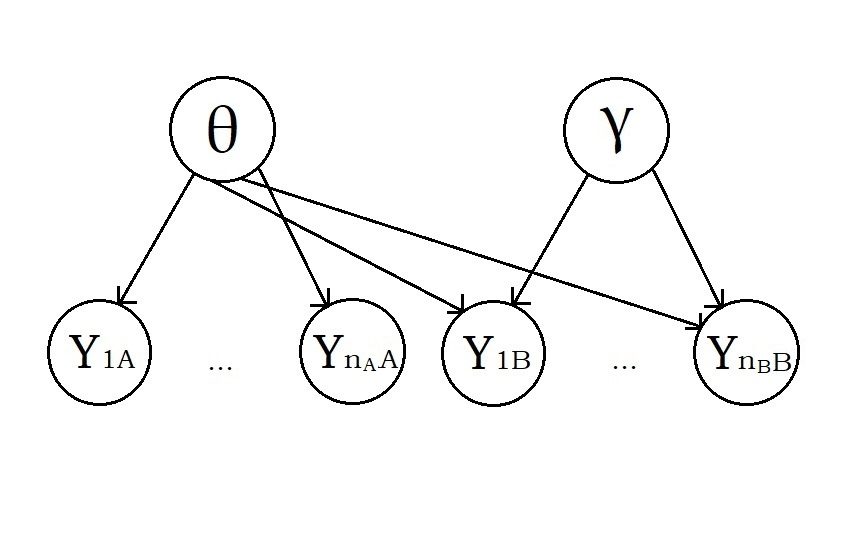
\includegraphics[scale=0.4]{img/esercizio6-01-grafo61.jpg}
\end{center}

Come si può osservare dallo schema, i figli di $\theta$ sono le osservazioni di A, quelle di B e $\gamma$ (questo perchè le osservazioni di B hanno come nodo padre anche $\gamma$). Inoltre $\theta$ non ha alcun nodo padre. \\
Quindi il Markov blanket risulta: \\
$bl(\theta)$ = $\lbrace Y_{1A}, Y_{2A} \ldots Y_{n_AA}, Y_{1B}, Y_{2B} \ldots Y_{n_BB}, \gamma\rbrace$.\\

Dunque\\
$p(\theta|y_{1A}, y_{2A} \ldots y_{n_AA}, y_{1B}, y_{2B} \ldots y_{n_BB}, \gamma) \propto$\\

$\propto p(\theta|a_\theta, b_\theta)$ $\prod_{i=1}^{n_A}{p(y_{iA}|\theta)} \prod_{j=1}^{n_B}{p(y_{jB}|\theta, \gamma)}$ =\\

$ = \frac{b_\theta^{a_\theta}}{\Gamma(a_\theta)}\theta^{a_\theta-1}e^{-b_\theta\theta} \prod_{i=1}^{n_A}{\frac{\theta^{y_{iA}} e^{-\theta}}{y_{iA}!}} \prod_{j=1}^{n_B}{\frac{(\theta\gamma)^{y_{jB}}e^{-\theta\gamma}}{y_{jB}!}}$ $\propto$\\

$\propto \theta^{a_\theta-1}e^{-b_\theta\theta}\theta^{\sum_{i=1}^{n_A}{y_{iA}}}e^{-n_A\theta}(\theta\gamma)^{\sum_{j=1}^{n_B}{y_{jB}}}e^{-n_B\theta\gamma}\simeq$\\

$\simeq \theta^{a_\theta + \sum_{i=1}^{n_A}{y_{iA}} + \sum_{j=1}^{n_B}{y_{jB}-1}}$ $ e^{-\theta(b_\theta+n_A+n_{B\gamma})}$

Da cui\\
$\theta|y_{1A},\ldots,y_{n_AA},y_{1B},\ldots,y_{n_BB}, \gamma \sim Gamma(a_\theta + \sum_{i=1}^{n_A}y_{iA} + \sum_{j=1}^{n_B}y_{jB}, b_\theta + n_A + n_{B}\gamma) $.\\


\item [c)]
Procediamo in modo simile al punto precedente, ricavando il Markov blanket di $\gamma$. \\ 
$\gamma$ non ha padre, e i suoi figli sono le osservazioni di B, che a loro volta hanno come genitore anche $\theta$ (come già detto). 
Dunque  il Markov blanket di $\gamma$ è $bl(\gamma)$ = $\lbrace  Y_{1B}, Y_{2B} \ldots Y_{n_BB}, \theta\rbrace$.\\


$p(\gamma|y_{1A}, y_{2A} \ldots y_{n_AA}, y_{1B}, y_{2B} \ldots y_{n_BB}, \theta) = $\\

$= p(\gamma|y_{1B}, y_{2B} \ldots y_{n_BB}, \theta) \propto $\\

$\propto p(\gamma|a_\gamma, b_\gamma)$ $\prod_{i=1}^{n_B}{p(y_{iB}|\theta,\gamma)} $ = \\

$= \frac{b_\gamma^{a_\gamma}}{\Gamma(a_\gamma)} \gamma^{a_\gamma-1}e^{-b_\gamma\gamma} \prod_{i=1}^{n_B}{\frac{(\theta\gamma)^{y_{iB}}e^{-\theta\gamma}}{y_{iB}!}} \propto $ \\

$\propto \gamma^{a_\gamma-1}e^{-b_\gamma\gamma}(\theta\gamma)^{\sum_{i=1}^{n_B}{y_{iB}}}e^{-n_B\theta_\gamma} \propto $ \\

$ \propto\gamma^{a_\gamma + \sum_{i=1}^{n_B}{y_{iB}-1} e^{-\gamma(b_\gamma+n_B\theta)}}$\\

Anche in questo caso possiamo riconoscere il kernel di una Gamma, perciò\\

$\gamma|y_{1A},\ldots,y_{n_AA},y_{1B},\ldots,y_{n_BB},\theta$ $\sim$ Gamma$(a_\gamma + \sum_{i=1}^{n_B}y_{iB} + b_\gamma + n_{B}\theta)$.\\

 
\item [d)] Riportiamo di seguito il codice R relativo all'algoritmo di Gibbs.

Come indicato nel testo dell'esercizio 4.8, i dataset utilizzati sono presenti nei file menchild30bach.dat
e menchild30nobach.dat.

Procediamo con l'inizializzazione dei dati:
\begin{verbatim}

>A<-c(1, 0, 0, 1, 2, 2, 1, 5, 2, 0, 0, 0, 0, 0,
+ 0, 1, 1, 1, 0, 0, 0, 1, 1, 2, 1, 3, 2, 0, 0,
+ 3, 0, 0, 0, 2, 1, 0, 2, 1, 0, 0, 1, 3, 0, 1,
+ 1, 0, 2, 0, 0, 2, 2, 1, 3, 0, 0, 0, 1, 1)

> B<-c(2, 2, 1, 1, 2, 2, 1, 2, 1, 0, 2, 1, 1, 2,
+ 0, 2, 2, 0, 2, 1, 0, 0, 3, 6, 1, 6, 4, 0, 3, 2, 0, 1,
+ 0, 0, 0, 3, 0, 0, 0, 0, 0, 1, 0, 4, 2, 1, 0, 0, 1, 0,
+ 3, 2, 5, 0, 1, 1, 2, 1, 2, 1, 2, 0, 0, 0, 2, 1,
+ 0, 2, 0, 2, 4, 1, 1, 1, 2, 0, 1, 1, 1, 1, 0, 2, 3, 2,
+ 0, 2, 1, 3, 1, 3, 2, 2, 3, 2, 0, 0, 0, 1, 0, 0,
+ 0, 1, 2, 0, 3, 3, 0, 1, 2, 2, 2, 0, 6, 0, 0, 0, 2, 0,
+ 1, 1, 1, 3, 3, 2, 1, 1, 0, 1, 0, 0, 2, 0, 2, 0,
+ 1, 0, 2, 0, 0, 2, 2, 4, 1, 2, 3, 2, 0, 0, 0, 1, 0, 0, 1,
+ 5, 2, 1, 3, 2, 0, 2, 1, 1, 3, 0, 5, 0, 0, 2,
+ 4, 3, 4, 0, 0, 0, 0, 0, 0, 2, 2, 0, 0, 2, 0, 0, 1, 1, 0,
+ 2, 1, 3, 3, 2, 2, 0, 0, 2, 3, 2, 4, 3, 3, 4,
+ 0, 3, 0, 1, 0, 1, 2, 3, 4, 1, 2, 6, 2, 1, 2, 2)

\end{verbatim}

Adesso effettuiamo l'inizializzazione dei parametri delle varie distribuzioni, poi settiamo il numero delle iterazioni da eseguire e il seed:

\begin{verbatim}
> a_theta<-2
> b_theta<-1
> v_gamma<-c(8, 16, 32, 64, 128)
> 
> n<-5000
> set.seed(150)
\end{verbatim}

Per la distribuzione gamma facciamo uso di un vettore perchè dobbiamo valutare i risultati per $a_\gamma$ = $b_\gamma \in \lbrace 8, 16, 32, 64, 128 \rbrace $.\\
Inizializziamo inoltre il vettore delle medie, il cui uso verrà chiarito a breve
\begin{verbatim}
> valori_medie<-NULL
\end{verbatim}

Nell'algoritmo di Gibbs viene eseguito un doppio ciclo: nel for più interno, per ognuna delle 5 coppie di iperparametri, vengono simulate le distribuzioni full conditionall (con 5000 valori sia per theta che per gamma); in ognuna delle iterazioni del for più esterno, vengono invece calcolati i valori attesi. \\ \\
Per comodità, facciamo uso di un array in 3 dimensioni: le prime due fanno riferimento a una matrice (5000 $\times$ 2) in cui vengono memorizzati i valori campionati di theta e gamma per ogni iterazione; la terza dimensione (5) serve per rieseguire questi passi, variando però gli iperparametri dell'a priori della distribuzione gamma.

\begin{verbatim}
> gibbs<-array(NA, c(n, 2, 5))
\end{verbatim}

Prima di eseguire l'algoritmo, calcoliamo, per ogni gruppo, le numerosità e i totali.
\begin{verbatim}
> nA<-length(A)
> nB<-length(B)
> 
> ytotA<-sum(A)
> ytotB<-sum(B)
> ytot<-ytotA+ytotB
\end{verbatim}

Tali valori caratterizzano i parametri delle full conditional.\\

Adesso inizializziamo i parametri gamma, theta e k: 
\begin{verbatim}
> gamma<-1
> theta<-1
> k<-1
\end{verbatim}

Come passo successivo, eseguiamo l'algoritmo:
\begin{verbatim}
> for(i in v_gamma){
+ a_gamma<-b_gamma<-i
+ for(j in 1:n){
+ theta<-rgamma(1, a_theta+ytot, b_theta+nA+nB*gamma)
+ gamma<-rgamma(1, a_gamma+ytotB, b_gamma+nB*theta)
+ gibbs[j,,k]<-cbind(theta, gamma)
+ }
+ k<-k+1
+   }
\end{verbatim}

Considerato che vogliamo ricavare il valore atteso della differenza tra thetaB e thetaA, dobbiamo calcolare la trasformazione theta*gamma-theta per ogni estrazione di theta e gamma ed eseguire la media su tutte le simulazioni. \\
Questo è possibile perchè abbiamo a disposizione il campione della congiunta a posteriori sia di theta che di gamma. \\
Ovviamente il procedimento deve essere ripetuto per ognuna delle 5 possibili scelte degli iperparametri della a priori di gamma, perciò memorizziamo i vari risultati nell'array valori\textunderscore medie.

\begin{verbatim} 
> for (i in 1:5){
+ valori_medie<-c(valori_medie, mean(gibbs[,1,i]*gibbs[,2,i]
+ -gibbs[,1,i]))
+  }
> valori_medie
[1] 0.3910311 0.3388716 0.2708131 0.2026279 0.1333113
\end{verbatim}

Come si può notare nell'output, il valore atteso della differenza tra thetaB e thetaA diminuisce 
progressivamente all'aumentare dei parametri dell'a priori di gamma. \\
Quindi, il numero di figli tra le due popolazioni prese in esame, decresce.

\begin{verbatim}
> leg<-v_gamma
> leg.txt<-rep("ab=bb",5)
> 
> par(mfrow=c(3,2))
> for(i in 1:5){
+ hist(gibbs[,1,i],prob=T,col="red",ylim=c(0,5),xlim=c(0,2.5),
+ ylab="densità a posteriori",xlab="numero medio di figli",main="")
+ lines(density(gibbs[,1,i]))
+ hist(gibbs[,1,i]*gibbs[,2,i],prob=T,col="blue",add=T)
+ lines(density(gibbs[,1,i]*gibbs[,2,i]))
+ }
> for(i in 1:5){
+ hist(gibbs[,1,i],prob=T,col="red",ylim=c(0,5),xlim=c(0,2.5),
+ ylab="densità a posteriori",xlab="numero medio di figli",main="")
+ lines(density(gibbs[,1,i]*gibbs[,2,i]))
+ hist(gibbs[,1,i]*gibbs[,2,i],prob=T,col="blue",add=T)
+ lines(density(gibbs[,1,i]*gibbs[,2,i]))
+ text(2, 4.5, paste("a_gamma=",lege[i]))
+ text(2, 3.5, paste("b_gamma=",lege[i]))
+ }
> 
\end{verbatim} 

\begin{center}
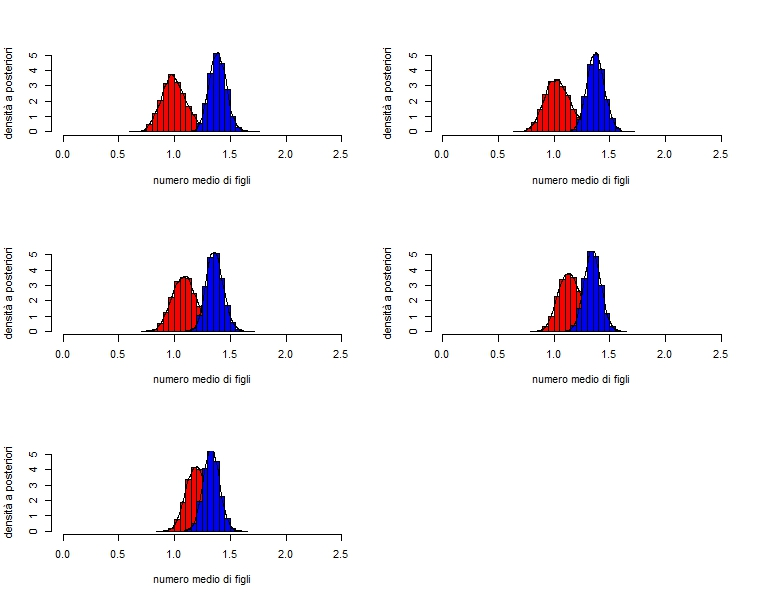
\includegraphics[scale=0.5]{img/esercizio6-01-grafo1.jpeg}
\end{center}

Quanto detto precedentemente, è evidente anche osservando i grafici.
La parte in rosso rappresenta thetaA, quella blu thetaB.
Come si può notare, le due distribuzioni sono sempre più vicine l'una all'altra all'aumentare degli iperparametri dell'a priori.

\begin{verbatim}
> x<-seq(0, 10, by=0.01)
> par(mfrow=c(1,1))
> plot(x, dgamma(x,8,8),type="l",xlim=c(0,5),ylim=c(0,5),
+ xlab=expression(gamma),ylab=expression(p(gamma)),
+ main="gamma a priori",col=1)


> for(j in 2:5){
+ curve(dgamma(x,v_gamma[j],v_gamma[j]),add=T,col=j)
+ }
> legend(2,4,c("a_gamma=b_gamma=8","a_gamma=b_gamma=16",
+ "a_gamma=b_gamma=32", "a_gamma=b_gamma=64",
+ "a_gamma=b_gamma=128"),col=c(1,2,3,4,5),lty=1)
\end{verbatim}

\begin{center}
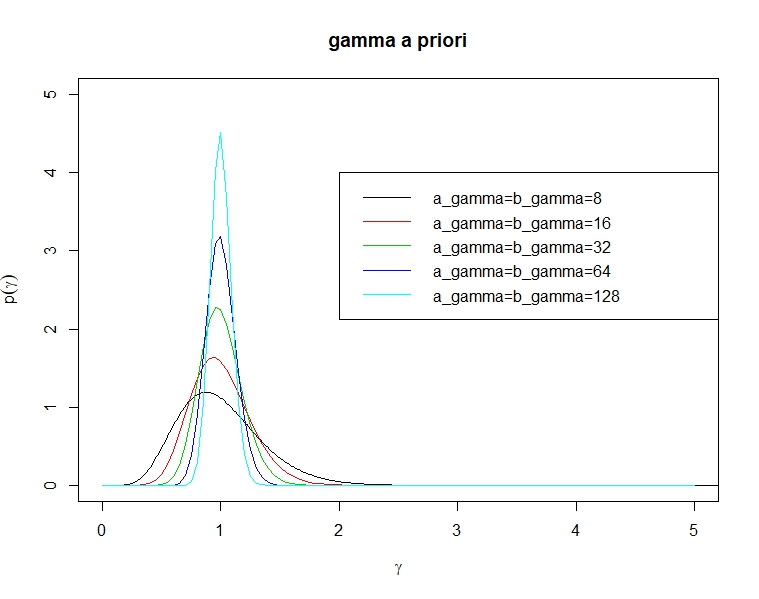
\includegraphics[scale=0.5]{img/esercizio6-01-grafo2.jpeg}
\end{center}

Osserviamo questo grafico: al crescere del numero degli iperparametri, l'apriori si "allunga" attorno a 1,
ossia il valore atteso.
Per quanto riguarda invece la varianza, questa risulta inversamente proporzionale al valore dei parametri.
Di conseguenza, la scelta degli iperparametri influisce molto sull'inferenza.
Più aumentano i valori di quest'ultimi, maggiore informazione è racchiusa nell'a priori: possiamo affermare ciò se consideriamo sia il cambiamento di tale distribuzione, sia il progressivo avvicinarsi di thetaA e thetaB.
Tenderemo quindi a ignorare thetaA e thetaB, e a fare affidamento solo sull'a priori.

\begin{verbatim}
> library(coda)
> effectiveSize(gibbs[,,1])

    var1     var2 
609.1041 605.4248 
\end{verbatim}

Con quest'ultime istruzioni, attraverso le quali possiamo calcolare l'effective size, siamo in grado di affermare che è stata raggiunta una condizione di equilibrio.


\end{enumerate}
% \newpage
% \subsection{Esercizio 7.2 - Hoff}

Unit information prior: Letting $ \Psi = \Sigma^{-1} $, show that a unit information prior for $(\boldsymbol{\theta},\Psi)$ is given by $\boldsymbol{\theta}|\Psi \sim $ multivariate normal $(\bar{\textbf{y}}, \Psi^{-1})$ and $\Psi \sim Wishart(p+1, \textbf{S}^{-1})$, where $\textbf{S} = \sum(\textbf{y}_i-\bar{\textbf{y}})(\textbf{y}_i-\bar{\textbf{y}})^{T}/n$. This can be done by mimicking the procedure outlined in Exercise 5.6 as follows:
\begin{enumerate}[label=\alph*)]
\item Reparameterize the multivariate normal model in terms of the precision matrix $\Psi = \Sigma^{-1}$. Write out the resulting log likelihood, and find a probability density $p_{U}(\boldsymbol{\theta},\Psi) = p_{U}(\boldsymbol{\theta}|\Psi)p_{U}(\Psi)$ such that $\log p(\boldsymbol{\theta},\Psi) = l(\boldsymbol{\theta},\Psi|\textbf{Y})/n+c$, where \textit{c} does not depend on $\boldsymbol{\theta}$ or $\Psi$.\\
Hint: Write $(\textbf{y}_i - \boldsymbol{\theta})$ as $(\textbf{y}_i - \bar{\textbf{y}}+\bar{\textbf{y}} - \boldsymbol{\theta})$, and note that $\sum\textbf{a}_i^T\textbf{Ba}_i$ can be written as tr(\textbf{AB}), where $\textbf{A} = \sum\textbf{a}_i\textbf{a}_i^T$.
\item Let $p_U(\Sigma)$ be the inverse-Wishart density induced by $p_U(\Psi)$. 
Obtain a density
$p_U(\boldsymbol{\theta},\Sigma|\textbf{y}_i,...,\textbf{y}_n)) \propto p_U(\boldsymbol{\theta}|\Sigma)p_U(\boldsymbol{\Sigma})p(\textbf{y}_i,...,\textbf{y}_n|\boldsymbol{\theta},\Sigma)$. 
Can this be interpreted as a posterior distribution for $\theta$ and $\Sigma$?
\end{enumerate}
\textbf{Svolgimento}\\

a) La distribuzione di probabilità di una normale multivariata è 
\begin{align*}
p(\textbf{Y}|\Sigma,\theta) = (2\pi)^{-1/2}|\Sigma|^{-1/2}\exp\left\{-1/2(\textbf{y}-\boldsymbol{\theta})^T\Sigma^{-1}(\textbf{y}-\boldsymbol{\theta})\right\}
\end{align*}
e riparametrizzando con $\Psi = \Sigma^{-1} $ avremo
\begin{align*}
p(\textbf{Y}|\Psi,\theta) = (2\pi)^{-p/2}|\Psi|^{1/2}\exp\left\{-1/2(\textbf{y}-\boldsymbol{\theta})^T\Psi(\textbf{y}-\boldsymbol{\theta})\right\}
\end{align*}

con relativa likelihood
\begin{align*}
\mathcal{L}(\textbf{Y}|\Psi,\theta) &= \prod_{i=1}^n(2\pi)^{-p/2}|\Psi|^{1/2}\exp\left\{-\frac{1}{2}(\textbf{y}_i-\boldsymbol{\theta})^T\Psi(\textbf{y}_i-\boldsymbol{\theta})\right\}\\
&\propto |\Psi|^{n/2}\exp\left\{-\frac{1}{2}\sum_{i=1}^n(\textbf{y}_i-\boldsymbol{\theta})^T\Psi(\textbf{y}_i-\boldsymbol{\theta})\right\}
\end{align*}

come suggerito dall'esercizio ci calcoliamo $\log p(\boldsymbol{\theta},\Psi) = l(\boldsymbol{\theta},\Psi|\textbf{Y})/n+c$

\begin{align*}
\log(\mathcal{L}(\textbf{Y}|\Psi,\theta)) &=  \frac{n}{2}\log|\Psi|\left\{-\frac{1}{2}\sum_{i=1}^n(\textbf{y}_i-\boldsymbol{\theta})^T\Psi(\textbf{y}_i-\boldsymbol{\theta})\right\}\\
\log(\mathcal{L}(\textbf{Y}|\Psi,\theta))/n + c &=  \frac{1}{2}\log|\Psi|\left\{-\frac{1}{2n}\sum_{i=1}^n(\textbf{y}_i-\boldsymbol{\theta})^T\Psi(\textbf{y}_i-\boldsymbol{\theta})\right\} + c
\end{align*}

Usando il suggerimento proposto dal testo avremo

\begin{align*}
-\frac{1}{2n}\sum_{i=1}^n(\textbf{y}_i-\boldsymbol{\theta})^T\Psi(\textbf{y}_i-\boldsymbol{\theta}) &= -\frac{1}{2n}\sum_{i=1}^n(\textbf{y}_i - \bar{\textbf{y}}+\bar{\textbf{y}} - \boldsymbol{\theta})^T\Psi(\textbf{y}_i - \bar{\textbf{y}}+\bar{\textbf{y}} - \boldsymbol{\theta})\\
&=-\frac{1}{2n}\sum_{i=1}^n\Big[(\textbf{y}_i - \bar{\textbf{y}})^T\Psi(\textbf{y}_i - \bar{\textbf{y}})\Big] -\frac{\cancel{n}}{2\cancel{n}} (\theta - \bar{\textbf{y}})^T\Psi(\theta- \bar{\textbf{y}})\\
&=-\frac{1}{2}tr(\textbf{S}\Psi)-\frac{1}{2}tr(\textbf{S}_\theta\Psi)
\end{align*}

Quindi la log likelihood calcolata al passo precedente diventerà

\begin{align*}
\log(\mathcal{L}(\textbf{Y}|\Psi,\theta))/n + c &=  \frac{1}{2}\log|\Psi|-\frac{1}{2}tr(\textbf{S}\Psi)-\frac{1}{2}tr(\textbf{S}_\theta\Psi) + c
\end{align*}

e tornando all'esponente avremo
\begin{align*}
\mathcal{L}(\textbf{Y}|\Psi,\theta)/n + c \propto  \underbrace{\exp\{|\Psi|\}-\exp\Big\{\frac{1}{2}tr(\textbf{S}\Psi)\Big\}}_\text{ $\sim$  Wishart($\Psi|$ k+2, $\textbf{S}^{-1}$)}
\underbrace{-\exp\Big\{\frac{1}{2}tr(\textbf{S}_\theta\Psi))\Big\}}_\text{ $\sim NM(\bar{\textbf{y}},\Psi^{-1})$}
\end{align*}

Abbiamo quindi trovato che $p_{U}(\boldsymbol{\theta},\Psi) = p_{U}(\boldsymbol{\theta}|\Psi)p_{U}(\Psi)$ dove 
\begin{align*}
p_{U}(\Psi) &= Wishart(\Psi| k+2, \textbf{S}^{-1}) \\ p_{U}(\boldsymbol{\theta}|\Psi) &= NM(\bar{\textbf{y}},\Psi^{-1})
\end{align*}


b) Da ciò che abbiamo appena calcolato al punto a), se volessimo tornare a $p_U(\Sigma)$ come suggerito dal testo avremo un Inverse Wishart e le relative distribuzioni di probabilità saranno

\begin{align*}
p_{U}(\Sigma) &\propto |\Sigma|^{-(p+k)/2}\exp\Big\{-\frac{1}{2}tr(S\Sigma^{-1})\Big\}\\
p_{U}(\boldsymbol{\theta}|\Sigma) &\propto \exp\Big\{-\frac{1}{2}(\boldsymbol{\theta} - \bar{\textbf{y}})^T\Sigma^{-1}(\boldsymbol{\theta}- \bar{\textbf{y}})\Big\}\\
p(\textbf{y}_i,...,\textbf{y}_n|\boldsymbol{\theta},\Sigma) &\propto |\Sigma|^{-n/2}\exp\Big\{-\frac{1}{2}\sum_{i=1}^n(\textbf{y}_i-\boldsymbol{\theta})^T\Sigma^{-1}(\textbf{y}_i-\boldsymbol{\theta})\Big\} \\
&\propto |\Sigma|^{-n/2}\exp\Big\{-\frac{1}{2}tr(S_1\Sigma^{-1})\Big\}
\end{align*}

volendo a questo punto trovare la densità chiesta, $p_U(\boldsymbol{\theta},\Sigma|\textbf{y}_i,...,\textbf{y}_n)) \propto p_U(\boldsymbol{\theta}|\Sigma)p_U(\boldsymbol{\Sigma})p(\textbf{y}_i,...,\textbf{y}_n|\boldsymbol{\theta},\Sigma)$, avremo

\begin{align*}
p_U(\boldsymbol{\theta},\Sigma|\textbf{y}_i,...,\textbf{y}_n)) &\propto |\Sigma|^{-n/2}|\Sigma|^{-(p+k)/2}\exp\Big\{-\frac{1}{2}tr[(S_1+S)\Sigma^{-1}] \Big\} \exp\Big\{-\frac{1}{2}(\boldsymbol{\theta} - \bar{\textbf{y}})^T\Sigma^{-1}(\boldsymbol{\theta}- \bar{\textbf{y}})\Big\}\\
&\propto \underbrace{|\Sigma|^{-\frac{n+p+k+1}{2}}\exp\Big\{-\frac{1}{2}tr[(S_1+S)\Sigma^{-1}] \Big\}}_\text{$\sim Inv-Wishart(n+k,(S+S_1)^{-1})$} \underbrace{|\Sigma|^{-1/2}\exp\Big\{-\frac{1}{2}(\boldsymbol{\theta} - \bar{\textbf{y}})^T\Sigma^{-1}(\boldsymbol{\theta}- \bar{\textbf{y}})\Big\}}_\text{$\sim N(\bar{y},\Sigma)$}
\end{align*}

che può essere interpretata come la distribuzioni a posteriori di $\boldsymbol{\theta}$ e $\Sigma$.

% \newpage
\section{Seconda Parte}
% \subsection{Esercizio 28 ottobre informatici}
Realizza un importance sampling per stimare il valore atteso della mistura di due beta $(0.3 \times \beta(5,2) + 0.7 \times \beta(2,8))$. Valuta altres\`i utilizzando il campione ottenuto la probabilit\`a di questa mistura nell'intervallo [0.45 - 0.55]

\textbf{Svolgimento}:
\bigskip

La funzione $g(x)$ usata campionare gli $x_i$ \`e una uniforme tra 0 ed 1.\\
Il codice R scritto per effettuare l'\textit{importance sampling} \`e il seguente:

\lstinputlisting[style=R]{code/es_19_oct_inf.R}

Il codice \`e una funzione che, data in input la dimensione del campione, effettua l' \textit{importance sampling} nella mistura restituendo il valore atteso sul campione e la probabilit\`a che si trovi nell'intervallo $[0.45 - 0.55]$.\\
Il valore atteso calcolato analiticamente dalla mistura \`e il seguente:
\begin{align*}
E [ 0.3 \times \beta (5,2) + 0.7 \times \beta (2,8) ] &=  	0.3 \times E [ \beta (5,2) ] + 0.7 \times E[\beta(2,8)] \\
&=  0.3 \times \dfrac{5}{7} + 0.7 \times \dfrac{2}{10} \\
&=  0.3542857 
\end{align*}
Invece qui di seguito sono presentati in forma tabellare i risultati ottenuti dall'esecuzione dello script al variare della dimensione del campione: \medskip \\
\begin{tabular}{|c|c|c|}
	\hline 
	Dimensione campione & Valore atteso & Probabilit\`a intervallo [0.45 - 0.55] \\ 
	\hline 
	10000 & 0.3560484 & 0.1990000 \\ 
	\hline 
	50000 & 0.3552311 & 0.2028800 \\ 
	\hline 
	100000 & 0.3552139 & 0.2034500 \\ 
	\hline 
\end{tabular} \medskip\\
Come possiamo notare il valore atteso calcolato tramite \textit{importance sampling} \`e abbastanza preciso in tutte e tre righe con un errore dell'ordine di $10^{-3}$ mentre la probabilit\`a di finire nell'intervallo [0.45 - 0.55] \`e sempre intorno allo 0.2 e ci\`o suggerisce che la densit\`a in questo intervallo \`e alta.
% \newpage
% \newcommand{\betaols}{\hat{\beta}_{ols}}

\subsection{Esercizio 13 Novembre 2017}
Dimostrare che $SSR_g$ (come definita a pagina 158 del libro di P. Hoff) tende a $SSR_{ols} = \sum(y_i - \betaols)^2$ per $g \rightarrow \infty$

\textbf{Svolgimento}:
\bigskip

Per poter dimostrare l'enunciato è necessaria la proprietà di idempotenza ovvero una matrice A è idempotente se $A^r = A \,\, \forall\, r \geqslant 1$ e sapere che $\betaols = X \left(X^T X \right)^{-1} X^T y$.\\
Innanzitutto risoliviamo il limite:
\begin{align*}
	lim_{g \rightarrow + \infty }\,\, SSR_g & = 	lim_{g \rightarrow + \infty } \,\, y^T \left(I - \dfrac{g}{g+1}  X \left(X^T X \right)^{-1} X^T \right) \\
	                                        & = y^T \left(I - X \left(X^T X \right)^{-1} X^T \right) y
\end{align*}
Possiamo notare che la proprietà di idempotenza vale per $X \left(X^T X \right)^{-1} X^T$ dato che
\begin{align*}
	\left[X \left(X^T X \right)^{-1} X^T\right]^2 = X \left(X^T X \right)^{-1} X^T \cdot X \left(X^T X \right)^{-1} X^T & = \\ X \left(X^T X \right)^{-1} \left[ X^T  X \left(X^T X \right)^{-1} \right] X^T  &=  X \left(X^T X \right)^{-1} X^T
\end{align*}
Perciò possiamo concludere la dimostrazione con i seguenti passaggi algebrici
\begin{align*}
	y^T \left(I - X \left(X^T X \right)^{-1} X^T \right) y & = y^T \left(I - X \left(X^T X \right)^{-1} X^T + X \left(X^T X \right)^{-1} X^T  - X \left(X^T X \right)^{-1} X^T \right) y \\ &= y^T \left(I - 2 X \left(X^T X \right)^{-1} X^T + X \left(X^T X \right)^{-1} X^T \right) y \\ &= y^T \left(I - 2 X \left(X^T X \right)^{-1} X^T + X \left(X^T X \right)^{-1} X^T X \left(X^T X \right)^{-1} X^T \right) y \\ &=
	y^Ty - 2 y^T X \left(X^T X \right)^{-1} X^T y + y^T X \left(X^T X \right)^{-1} X^T X \left(X^T X \right)^{-1} X^T y                                                                  \\ &=
	y^Ty - 2 \betaols^T X^T  y + \betaols^T X^T X \betaols                                                                                                                               \\ &= \sum_{i=1}^{n}(y_i - \betaols^T x_i)^2
\end{align*}
che è ciò che volevamo dimostrare
% \newpage
% \subsection{Soluzione esercizio 8.2 Hoff}

Sensitivity analysis: In this exercise we will revisit the study from Exercise 5.2, in which 32 students in a science classroom were randomly assigned to one og two study methods, A and B, with $n_A = n_B = 16$. After several weeks of study, students were examined on the course material, and the scores are summarized by $\{\bar{y}_A = 75.2, s_A = 7.3\}, \{\bar{y}_B = 77.5, s_B = 8.1\}$. We will estimate $\theta_A = \mu+\delta$ and $\theta_B = \mu-\delta$ using the two-sample model and prior distributions of Section 8.1.
\begin{itemize}
	\item[a)] Let $\mu \sim $normal(75,100),  $1/\sigma^2\sim$ gamma(1,100) and $\delta\sim$normal$(\delta_0, \tau^2_0)$. For each combination of $\delta_0 \in \{-4, -2, 0, 2, 4\}$ and $\tau_0 \in \{10, 50, 100, 500\}$, obtain the posterior distribution of $\mu$, $\delta$ and $\sigma^2$ and compute
	\begin{itemize}
		\item[i.] Pr$(\delta>0|\boldsymbol{Y})$;
		\item[ii.] a 95$\%$ posterior confidence interval for $\delta$;
		\item[iii.] the prior and posterior correlation of $\theta_A$ and $\theta_B$.
	\end{itemize}
	\item[b)] Describe how you might use these results to convey evidence that $\theta_A<\theta_b$ to people of a variety of prior opinions.
\end{itemize}

\textbf{Svolgimento}
\bigskip

L'obiettivo di questo esercizio è quello di condurre un'analisi di sensitività. 
Ossia, si vuole valutare il cambiamento dell'inferenza al variare della specifica\-zione della prior. 
Dato il modello delle osservazioni:
\[
Y_{iA} = \mu + \delta + \varepsilon_{iA};
\]
\[
Y_{iB} = \mu - \delta + \varepsilon_{iB} = \varepsilon_{iB};
\]
\[
\varepsilon_{ij} | \sigma^2 \sim i.i.d \quad N(0,\sigma^2) \quad j = A,B;
\]
\[
\mu|\gamma_0^2,\mu_0 \sim N(\mu_0,\gamma_0^2);
\]
\[
\mu|\tau_0^2,\delta_0 \sim N(\delta_0,\tau_0^2);
\]
\[
\sigma^2 | \nu_0,\sigma_0^2 \sim inverse-Gamma(\frac{\nu_0}{2},\frac{\nu_0\sigma^2}{2})
\]
\[
p(\mu,\delta,\sigma^2) = p(u)p(\delta)p(\sigma^2)
\]
e la sua rappresentazione tramite DAG qui di seguito:

\begin{tikzpicture}[
	> = stealth, % arrow head style
	shorten > = 1pt, % don't touch arrow head to node
	auto,
	node distance = 3cm, % distance between nodes
	semithick
]

\tikzstyle{every state}=[
	draw = black,
	thick,
	fill = white,
	minimum size = 4mm
]

\node[state, dashed] (v1)  {$\mu$};

\node[state] (y1) [below left of= v1] {$y_{1A}$};
\node[state] (y2) [right of= y1] {$y_{1A}$};
\node[state] (y3) [right of= y2] {$y_{naA}$};
\node[state] (y4) [right of= y3] {$y_{1B}$};
\node[state] (y5) [right of= y4] {$y_{2B}$};
\node[state] (y6) [right of= y5] {$y_{nbB}$};

\node[state, dashed] (v2) [above right of=y4] {$\theta$};

\node[state, dashed] (s1) [below right=1cm and 0.8cm of y3] {$\sigma^2$};

\path[->] (v1) edge node {} (y1);
\path[->] (v1) edge node {} (y2);
\path[->] (v1) edge node {} (y3);
\path[->] (v1) edge node {} (y4);
\path[->] (v1) edge node {} (y5);
\path[->] (v1) edge node {} (y6);

\path[->] (v2) edge node {} (y1);
\path[->] (v2) edge node {} (y2);
\path[->] (v2) edge node {} (y3);
\path[->] (v2) edge node {} (y4);
\path[->] (v2) edge node {} (y5);
\path[->] (v2) edge node {} (y6);

\path[->] (s1) edge node {} (y1);
\path[->] (s1) edge node {} (y2);
\path[->] (s1) edge node {} (y3);
\path[->] (s1) edge node {} (y4);
\path[->] (s1) edge node {} (y5);
\path[->] (s1) edge node {} (y6);

\draw[black, dotted] (2.3, -2.2) -- (2.8, -2.2);
\draw[black, dotted] (10.9, -2.2) -- (11.4, -2.2);
\end{tikzpicture}

\begin{itemize}[-]
\item Assegniamo agli iperparametri i valori che sono stati richiesti
\[
\mu_0 = 75; \quad \gamma_0^2 = 100; \quad \frac{\nu}{2} = 1 \implies \nu_0 = 2; \quad \frac{\nu_0\sigma_0^2}{2}=100
\]
\[
\implies \sigma_0^2 = 100;
\]
\[
\delta_0 \in \{-4,-2,0,2,4\}; \quad \tau_0^2 \in \{10,50,100,500\}
\]
avendo i seguenti dati campionari
\[
\bar{y_A} = 75.2, \quad s_A = 7.3, n_A = 16;
\]
\[
\bar{y_B} = 77.5, \quad s_B = 8.1, n_B = 16;
\]
\[
n_j=n=16; \quad \bar{y_j}=\frac{1}{n_j}\sum_{i=1}^{n_j}y_{ij}; \quad s_j = \sqrt{\frac{1}{n_j-1}\sum_{i=1}^{n_j}(y_{ij}-\bar{y_j})^2}
\]
per fare l'inferenza richiesta è necessario determinare la distribuzione a posteriori delle variabili $\mu,\delta,\sigma^2$, ossia
$$p(\mu,\delta,\sigma^2|y_{1A},\dots,y_{n_AA},y_{1B},\dots,y_{n_BB}).$$ 
Per far ciò approssimiamo tale distribuzione mediante campionamento MCMC, secondo l'ottica Gibbs. Le distribuzioni full conditional dei parametri sono quindi le seguenti:
\[
\sigma^2 | y_{1A},\dots,y_{n_AA},y_{1B},\dots,y_{n_BB}, \mu, \delta \sim inverse-Gamma(\frac{\nu_n}{2},\frac{\nu_n\sigma_n^2}{2}) 
\]
in cui 
\[
\nu_n = \nu_0 + n_A + n_B;
\]
\[
\nu_n \sigma_n^2=\nu_0\sigma_0^2+\sum_{i=1}^{n_A}[y_{iA}-(\mu+\delta)]^2+ \sum_{k=1}^{n_B}[y_{kB}-(\mu-\delta)]^2=
\]
\[
=\nu_0\sigma_0^2 + \sum_{i=1}^{n_A}[y_{iA}^2-2(\mu+\delta)y_{iA} + (\mu + \delta)^2] +
\]
\[
 +\sum_{k=1}^{n_B}[y_{kB}^2-2(\mu-\delta) + (\mu - \delta)^2]=
\]
\[
=\nu_0\sigma_0^2 + \sum_{i=1}^{n_A}y_{iA}^2 - 2(\mu + \delta)\sum_{i=1}^{n_A}y_{iA} + n_A(\mu + \delta)^2+ 
\]
\[
+ \sum_{k=1}^{n_B}y_{kB}^2 - 2(\mu-\delta)\sum_{k=1}^{n_B}y_{kB} + n_B(\mu-\delta)^2=
\]
\[
\nu_0\sigma_0^2+(n_A-1)s_A^2+n_A\bar{y}_A^2-2(\mu + \delta)n_A\bar{y}_A+n_{A}(\mu+\delta)^2+
\]
\[
+(n_B-1)s_B^2+n_B\bar{y}_B^2-2(\mu-\delta)n_B\bar{y}_B+n_B(\mu-\delta)^2=
\]
\[
+n_B(\mu-\delta)^2=\nu_0\sigma_0^2 +(n-1)(s_A^2+s_B^2)+n(\bar{y}_A^2+\bar{y}_B^2)+
\]
\[
+n[-2(\mu+\delta)\bar{y}_A+(\mu+\delta)^2-2(\mu-\delta)\bar{y}_B+(\mu-\delta)^2=
\]
\[
\nu_0\sigma_0^2+(n-1)(s_A^2+s_B^2)+n(\bar{y}_A^2+\bar{y}_B^2)+
\]
\[
+2n[-\mu(\bar{y}_A+\bar{y}_B)+\delta(\bar{y}_B-\bar{y}_A)+\mu^2 + \delta^2].
\]
\[
\mu|y_{1A},\dots,y_{nA},y_{1B},\dots,y_{nB},\delta,\sigma^2 \sim N(\mu_n,\gamma_n^2)
\]
in cui 
\[
\gamma_n^2=[\frac{1}{\gamma_0^2}+\frac{(n_A+n_B)}{\sigma^2}]^{-1} = \frac{\gamma_0\sigma^2}{\sigma^2+(n_A+n_B)\sigma_0^2};
\]
\[
\mu_n =\gamma_n^2[\frac{\mu_0}{\gamma_0^2}+\frac{1}{\sigma^2}\sum_{i=1}^{n_A}(y_{iA}-\delta)+\frac{1}{\sigma^2}\sum_{k=1}^{n_B}(y_{kB}+\delta)]= 
\]
\[
=\gamma_n^2[\frac{\mu_0}{\gamma_0^2}+\frac{1}{\sigma^2}[(\sum_{i=1}^{n_A}y_{iA}) - n_A\delta + (\sum_{k=1}^{n_B}y_{kB} + n_B\delta)]]=
\]
\[
= \gamma_n^2[\frac{\mu_0}{\gamma_0^2}+\frac{1}{\gamma^2}(n_A\bar{y}_A-n_A\delta+n_B\bar{y}_B+n_B\delta)] = 
\]
\[
=\gamma_n^2[\frac{\mu_0}{\gamma_0^2}+\frac{n}{\sigma^2}(\bar{y}_A+\bar{y}_B)].
\]
\[
\delta | y_{1A},\dots,y_{n_aA},y_{1B},\dots,y_{n_BB},\mu,\delta^2 \sim N(\delta_n,\tau_n^2)
\]
in cui
\[
\tau_n^2 = (\frac{1}{\tau_0^2}+\frac{n_A+n_B}{\sigma^2})^{-1} = \frac{\sigma^2\tau_0^2}{\sigma^2+(n_A+n_B)\tau_0^2};
\]
\[
\delta_n = \tau_n^2[\frac{\delta_0}{\tau_0^2}+\frac{1}{\sigma^2}\sum_{i=1}^{n_A}(y_{iA}-\mu)-\frac{1}{\sigma^2}\sum_{k=1}^{n_B}(y_{kB}-\mu)]=
\]
\[
\tau_n^2[\frac{\delta_0}{\tau_0^2}+\frac{1}{\sigma^2}[(\sum_{i=1}^{n_A}y_{iA}-n_A\mu)+(\sum_{k=1}^{n_B}y_{kB}-n_B\mu)]]=
\]
\[
\tau_n^2[\frac{\delta_0}{\tau_0^2}+\frac{1}{\delta^2}(n_A\bar{y_A}-n_A\mu-n_B\bar{y_B})+n_B\mu)]=\tau_n^2[\frac{\delta_0}{\tau_0^2}+\frac{n}{\sigma^2}(\bar{y_A}-\bar{y_B})].
\]
Di seguito viene mostrato il codice R che svolge i punti a i), a ii) e a iii). Prima però viene calcolata la correlazione a priori tra $\theta_A$ e $\theta_B$ per il punto a iii):
\[
Corr(\theta_A,\theta_B) = \frac{Cov(\theta_a,\theta_B)}{\sqrt{Var(\theta_A)Var(\theta_B)}} = \frac{Cov(\mu+\delta,\mu-\delta)}{\sqrt{Var(\mu+\delta)Var(\mu-\delta)}}=
\]
\[
= \frac{Cov(\mu,\mu)+Cov(\mu,\delta)-Cov(\mu,\delta)-Cov(\delta,\delta)}{\sqrt{(Var(\mu)+Var(\delta))(Var(\mu)+Var(\delta))}}=
\]
\[
\frac{Var(\mu)-Var(\delta)}{\sqrt{(Var(\mu)+Var(\delta))^2}}
=\frac{\gamma_0^2-\tau_0^2}{\gamma_0^2+\tau_0^2}
\]
e quindi
\[
 \begin{matrix}
  \tau_0^2 & 10 & 50 & 100 & 500 \\
  Corr(\theta_A,\theta_B) & 0.81 & 0.33 & 0 & -0.67
 \end{matrix}
\]

\begin{lstlisting}[style=R]
#Quantita' campionarie a disposizione per i due
#gruppi (medie, deviazioni standard e numerosita'):
y.barA<-75.2
y.barB<-77.5
sA<-7.3
sB<-8.1
nA<-nB<-n_<-16

#Setting iperparametri delle prior: gli iperparametri 
#media e varianza(rispettivamente chiamati delta0 e tau20) 
#per la a priori di delta, la semidifferenza tra
#le medie dei due gruppi, sono due vettori dal momento
#che l'obbiettivo dell' esercizio e' quello di valutare se 
#e come cambia l'inferenza a seconda della prior specificata 
#proprio su delta.

delta0<-c(-4 ,-2 ,0 ,2 ,4)
tau20<-c(10, 50, 100, 500)
mu0<-75
gamma20<-100
v0<-2
sigma20<-100

#Valori iniziali dei parametri e numero di simulazioni:

delta <-(y.barA-y.barB)/2
mu<-(y.barA+y.barB) /2

nsimul<-1000

#Creiamo un array dei i valori campionati durante l'algoritmo:

gibbs<-array(NA,c(nsimul,3,length(delta0)*length(tau20)))

#Ciclo Gibbs:

v<-1
for(j in delta0){
	for(k in tau20){
		for(i in 1:nsimul) {

#Aggiorniamo sigma:

			vn<-v0+nA+nB
			vnsigma2n<-v0*sigma20+(n_-1)*(sA^2+sB^2)+n_*(y.barA^2+y.barB^2)+2*n_*(mu^2
			delta^2-mu*(y.barA+y.barB)+delta*(y.barB-y.barA))
			sigma2<-1/rgamma(1,vn /2,vnsigma2n/2)

#Aggiorniamo mu:

			gamma2n<-gamma20*sigma2/(sigma2+(nA+nB)*gamma20)
			mun<-gamma2n*(mu0/gamma20+n_*(y.barA+y.barB)/sigma2)
			mu<-rnorm(1,mun,sqrt(gamma2n))

#Aggiorniamo delta:

			tau2n<-k*sigma2 /(sigma2+(nA+nB)*k)
			deltan<-tau2n*(j/k+n_*(y.barA-y.barB)/sigma2)
			delta<-rnorm(1,deltan,sqrt(tau2n))

			gibbs[i,,v]<-c(mu,delta,sigma2)
		}
		v<-v+1
	}
}

colnames(gibbs)<-c("mu","delta","sigma2")

#a)

probabilita.post<-corrrelazione. post<-matrix (NA,5,4)
quantili.post<-NULL
v=1
for(i in 1:5){
  for(j in 1:4){
    probabilita.post[i,j]<-mean(gibbs[,2,v]<0)
    quantili.post<-rbind(quantili.post,quantile(gibbs[,2,v],c(0.025,0.975)))
    correlazione.post[i,j]<-cor(gibbs[,1,v]+gibbs[,2,v],
    gibbs[,1,v]-gibbs[,2,v])
    v<-v+1
  }
}

rownames(probabilita.post)<-rownames(correlazione.post)<-
c("delta0=-4",+"delta0=-2","delta0=0","delta0=2","delta0=4")
colnames(probabilita.post)<-colnames(correlazione.post)<-
c("tau20=10",+" tau20=50"," tau20=100"," tau20=500")
rownames(quantili.post)<-c("delta0=-4 tau20=10"," delta0=-4 tau20=50",
"delta0=-4 tau20=100","delta0=-4 tau20=500","delta0=-2 tau20=10",
"delta0=-2 tau20=50","delta0=-2 tau20=100","delta0=-2 tau20=500",
"delta0=0 tau20=10","delta0=0 tau20=50","delta 0=0 tau20=100",
"delta0=0 tau20=500","delta0=2 tau20=10","delta0=2 tau20=50",
"delta0=2 tau20=100","delta0=2 tau20=500","delta0=4 tau20=10",
"delta0=4 tau20=50","delta0=4 tau20=100","delta0=4 tau20=500")

#i)

probabilita.post
\end{lstlisting}

{
\color{red}
\begin{Verbatim}
> probabilita.post
          tau20=10    tau20=50  tau20=100  tau20=500
delta0=-4    0.899     0.834      0.807      0.802
delta0=-2    0.841     0.812      0.778      0.788
delta0=0     0.755     0.802      0.772      0.786
delta0=2     0.704     0.769      0.788      0.799
delta0=4     0.617     0.756      0.771      0.781
\end{Verbatim}
}
La tabella precedente contiene la probabilità a posteriori che la semidif\-ferenza tra le medie dei due gruppi sia negativa, 
per ciascuna delle possibile coppie di valori di $\delta_0$ e $\tau_o^2$.

\begin{lstlisting}[style=R]
#Rappresentiamo tutte queste probabilita' anche graficamente:

par(mfrow=c(3,2))
for(i in 1:5){
  plot(tau20,probabilita.post[i,],pch=20, xlab=expression(tau^2[0]),
  ylab=expression(p(delta<0 given bold(Y)), type="l")
  legend("right",paste("delta0=",delta0[i]), bty="n")
}

\end{lstlisting}

\begin{figure}[!ht]
 \centering
 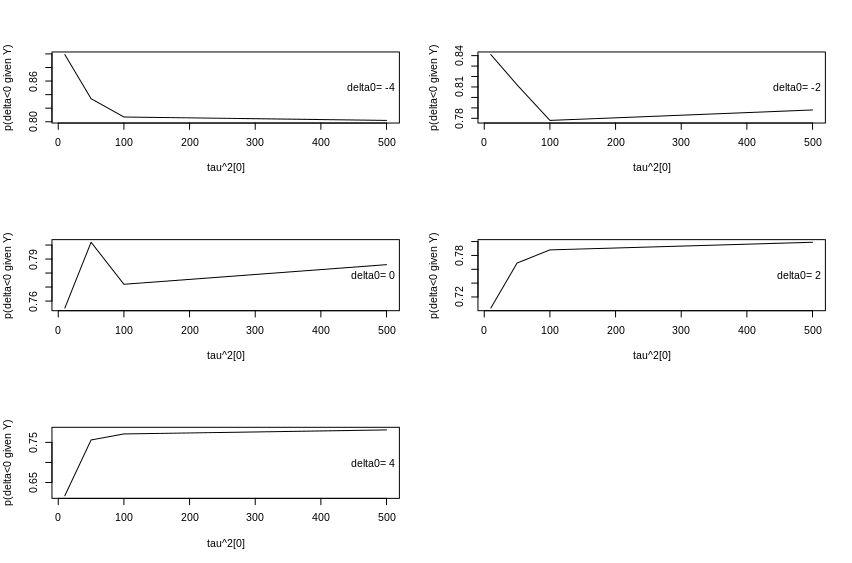
\includegraphics[scale = 0.7]{img/esercizio8-2-1}
 \caption{probabilità a posteriori al variare della prior}
 \label{figure:figura12}
\end{figure}
\newpage
\begin{lstlisting}[style=R]
#a)ii
\end{lstlisting}
{
\color{red}
\begin{Verbatim}
> quantili.post
                        2.5%    97.5%
delta0=-4 tau20=10  -4.166501 0.885176
delta0=-4 tau20=50 -4.080470 1.261487
delta0=-4 tau20=100 -3.966220 1.815875
delta0=-4 tau20=500 -3.984476 1.560537
delta0=-2 tau20=10  -3.921579 1.224411
delta0=-2 tau20=50  -3.987036 1.520727
delta0=-2 tau20=100 -3.956075 1.720433
delta0=-2 tau20=500 -3.794180 1.702581
delta0=0 tau20=10   -3.459266 1.618012
delta0=0 tau20=50   -3.884302 1.613191
delta 0=0 tau20=100 -4.000856 1.521053
delta0=0 tau20=500  -4.081757 1.850854
delta0=2 tau20=10   -3.017789 1.890537
delta0=2 tau20=50   -3.727812 1.800686
delta0=2 tau20=100  -3.664780 1.952699
delta0=2 tau20=500  -4.089526 1.830220
delta0=4 tau20=10   -2.637665 2.135446
delta0=4 tau20=50   -3.850333 1.857685
delta0=4 tau20=100  -3.661231 1.695296
delta0=4 tau20=500  -4.298413 1.823357
\end{Verbatim}
}

\begin{lstlisting}[style=R]
#a)iii

#Confrontiamo ora le correlazioni a priori e quelle a
#posteriori fra le medie dei due gruppi thetaA=mu+delta e 
#thetaB=mu-delta.

correlazione.prior<-c(0.81,0.33,0,-0.67)

#Le correlazioni a posteriori precedentemente calcolate invece sono:
}

\end{lstlisting}

{
\color{red}
\begin{Verbatim}
> correlazione.post
              tau20=10    tau20=50    tau20=100    tau20=500
  delta0=-4 0.11470736  0.04394125 -0.014843283 -0.047380931
  delta0=-2 0.05693164  0.04900340 -0.081550575 -0.007036669
  delta0=0  0.06714184  0.03791250 -0.008966994 -0.026858228
  delta0=2  0.11899453  0.04389222 -0.009447653 -0.044961021
  delta0=4  0.13144920 -0.03688193  0.005192835 -0.064853163
\end{Verbatim}
}


\begin{lstlisting}[style=R]
#b)

win.graph()
par(mfrow=c(2,2))
x<-seq(-50,50,by=0.01)
v<-0
for(j in 1:4){
  plot(x,dnorm(x,delta0[1],sqrt(tau20[j])), xlim=c(-10,10),ylim=c(0,0.3),
  xlab=expression(delta),ylab="density",type="l",col="grey")
  lines(density(gibbs[,2,j]))
  legend("topright",legend=c("posterior","prior"),lwd=c(2,2),col=c("black",
  "gray"),bty="n")
  text(5.5,0.15,paste("tau20=",tau20[j]))
}

win.graph()
par(mfrow=c(2,2))
x<-seq(-50,50,by=0.01)
v<-0
for(j in 1:4){
  plot(x,dnorm(x,delta0[5],sqrt(tau20[j])),xlim=c(-10 ,10),ylim=c(0,0.3),
  xlab=expression(delta),ylab="density",type="l",col="grey")
  lines(density(gibbs[,2,j+16]))
  legend("topright",legend=c("posterior","prior"),lwd=c(2,2),col=c("black",
  "gray"),bty="n")
  text(5.5,0.15, paste("tau20=",tau20[j]))
}

\end{lstlisting}
\begin{figure}
 \centering
 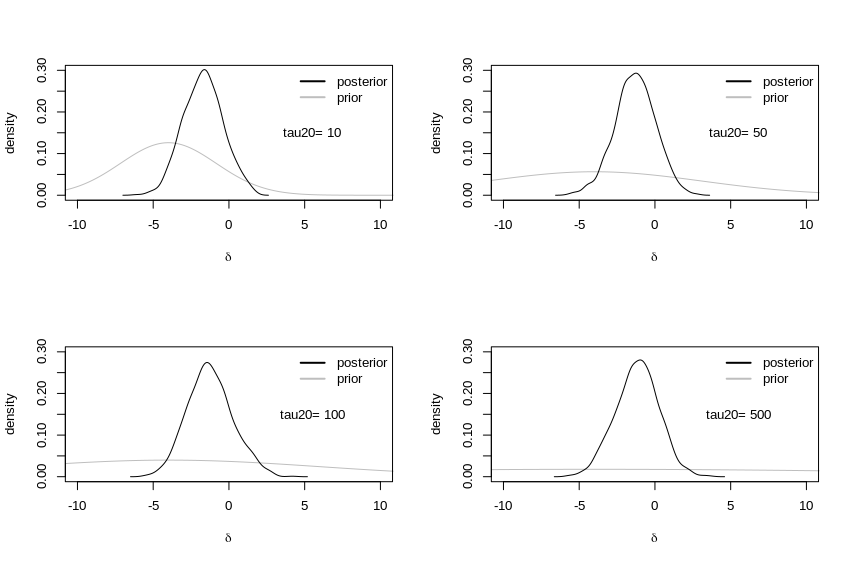
\includegraphics[scale=0.7]{img/esercizio8-2-2}
 \caption{densita' a posteriori al variare della prior}
 \label{figure:figura13}
\end{figure}

\begin{figure}
 \centering
 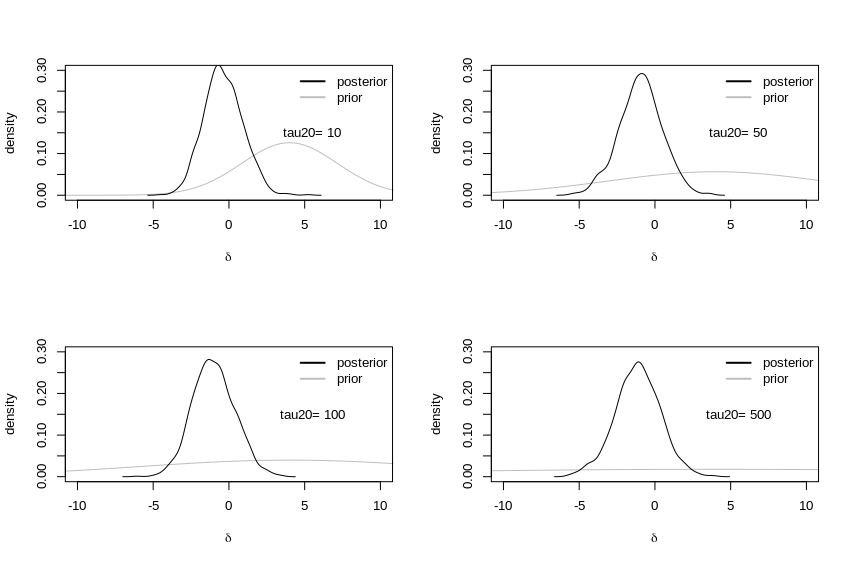
\includegraphics[scale=0.7]{img/esercizio8-2-3}
 \caption{densita' a posteriori al variare della prior}
 \label{figure:figura14}
\end{figure}

\begin{lstlisting}[style=R]
#Facciamo una veloce verifica della convergenza dell'algoritmo:
#library(coda)
effectiveSize(gibbs[,,1])
\end{lstlisting}

{
\color{red}
\begin{Verbatim}
  mu  delta  sigma2
1000   1000    1000
\end{Verbatim}
}

\end{itemize}


% \newpage
% \subsection*{Esercizio 10.2 Hoff} % (fold)

Nesting success: younger male sparrows may or may not nest during a mating season, perhaps depending on their physical characteristics. Researchers have recorded the nesting success of 43 young male sparrows of the same age, as well as their wingspan, and the data appear in the file \texttt{msparrownest.dat}. Let $Y_i$ be the binary indicator that sparrow $i$ successfully nests, and let $x_i$ denote their wingspan. Our model for $Y_i$ is $logit\theta(Y_i = 1|\alpha, \beta, x_i)) = \alpha + \beta x_i$, where the logit function is given by $logit \theta = log\left[\frac{\theta}{1-\theta}\right]$.
\begin{enumerate}
  \item Write out the joint sampling distribution  $\prod_{i=1}^{n}p(y_i | \alpha, \beta, x_i)$ and simplify as much as possible.
  \item Formulate a prior probability distribution over $\alpha$ and $\beta$ by considering the range of $Pr(Y = 1|\alpha,\beta,x)$ as x ranges over $10$ to $15$, the approximate range of the observed wingspans.
  \item Implement a Metropolis algorithm that approximates $p(\alpha, \beta|\mathbf{y}, \mathbf{x})$. Adjust the proposal distribution to achieve a reasonable acceptance rate, and run the algorithm long enough so that the effective sample size is at least $1,000$ for each parameter.
  \item Compare the posterior densities of $\alpha$ and $\beta$ to their prior densities.
  \item Using output from the Metropolis algorithm, come up with a way to make a confidence band for the following function $f_{\alpha\beta}(x)$ of wingspan:
  $$f_{\alpha\beta}(x) = \frac{e^{\alpha + \beta x}}{1+e^{\alpha + \beta x}}$$
  where $\alpha$ and $\beta$ are the parameters in your sampling model. Make a plot of such a band.
\end{enumerate}


\textbf{Svolgimento}:
\bigskip

L'esercizio ha come obiettivo principale quello di studiare la relazione tra laprobabilità di nidificare e l'ampiezza delle ali per un gruppo di $43$ uccellini maschi della stessa età. Il setting del modello è il seguente:
$$Y_i = \begin{cases} 1, & \mbox{se l'uccellino } i\mbox{ nidifica} \\ 0, & \mbox{altrimenti } \end{cases}; \quad x_i = \text{ampiezza dell'uccellino } i; \quad i = 1, \dots, 43$$
La verosomiglianza per ogni singola osservazione è pertanto una Bernoulli:
$$p(y_i | p_i) = p_i^{y_i}(1-p_i)^{1-y_i}$$
Studiamo la relazione tra la probabilità di nidificare e l'ampiezza delle ali con il modello logistico (siamo quindi nell'ambito dei modelli lineari generalizzati):
$$g(p_i) = logit(p_i) = log\left(\frac{p_i}{1-p_i}\right) = \eta_i = \alpha + \beta x_i$$
pertanto
$$g^{-1}(\eta_i) = p_i = \frac{e^{\eta_i}}{1+e^{\eta_i}} = \frac{e^{\alpha + \beta x_i}}{1+e^{\alpha + \beta x_i}}$$
\subsubsection*{Parte a} 
Scriviamo la verosomiglianza secondo il modello appena descritto, quindi come funzione di $\alpha$ e $\beta$ (ricordiamo l'indipendenza condizionata a tali parametri):
\begin{gather}
\nonumber\mathcal{L}(\alpha;\beta;\mathbf{y};\mathbf{X}) = p(\mathbf{y}|\alpha, \beta, \mathbf{X}) = \prod_{i=1}^{n}p(y_i |\alpha, \beta, \mathbf{x_i}) = \prod_{i=1}^{n}\left[\left(\frac{e^{\eta_i}}{1+e^{\eta_i}}\right)^{y_i}\left(\frac{1}{1+e^{\eta_i}}\right)^{1-y_i}\right] \\
\nonumber=\prod_{i=1}^{n} \frac{e^{y_i\eta_i}}{1+e^{\eta_i}} = \prod_{i=1}^{n}(e^{y_i\eta_i} - log(1-e^{\eta_i})) = e^{\sum_{i=1}^{n}[y_i\eta_i - log(1+e^{\eta_i})]} \\
\nonumber=e^{\sum_{i=1}^{n}[y_i(\alpha+\beta x_i) - log(1+e^{\alpha+\beta x_i})]}
\end{gather}
Potevamo in maniera analoga procedere passando direttamente attraverso la scrittura delle singole verosomiglianze nella forma della famiglia esponenziale in questo modo:
$$p(y_i|p_i) = p_i^{y_i}(1-p_i)^{1-y_i} = e^{y_i log(\frac{p_i}{1-p_i}+log(1-p_i))}$$
pertanto
\begin{gather}
\nonumber \prod_{i=1}^{n} p(y_i|p_i) = \prod_{i=1}^{n} e^{\sum_{i=1}^{n}[y_i \eta_i + log(\frac{1}{1+\eta_i})]} = e^{\sum_{i=1}^{n}[y_i \eta_i + log(1+\eta_i)]}\\
\nonumber e^{\sum_{i=1}^{n}[y_i(\alpha+\beta x_i) - log(1+e^{\alpha+\beta x_i})]}
\end{gather}
\subsubsection*{Parte b} % (fold)
Possiamo formulare la a priori per $\alpha$ e $\beta$ in molti modi, due dei quali sono i seguenti:
\begin{enumerate}
  \item \textbf{soggettivamente:} a priori pensiamo che la probabilità di nidificare sia alta e che vari tra $[0.5, 0.9]$; sapendo inoltre che il campo di variazione della covariata è $[10, 15]$, troviamo il range di $\alpha$ e $\beta$ che sia compatibile conq uello della probabilità e in base ad esso formuliamo la prior sui parametri. In dettaglio: Pensiaom che $p=Pr(Y=1 | \alpha, \beta, \mathbf{x}) \in [0.5, 0.9]$ e quindi che $logit(p) = log\left(\frac{p}{1-p}\right) = \alpha + \beta x \in [0, 2.2]$. Si ha il seguente sistema di disequazioni:
  $$\begin{cases} \alpha+\beta x \geq 0 \\ \alpha + \beta x \leq 2.2 \end{cases}$$
  Troviamo il range di $\alpha$ e di $\beta$ risolvendo il sistema per il valore minimo e per quello massimo di x:
   $$\begin{cases} \alpha+10\beta = 0 \\ \alpha +  15\beta = 2.2 \end{cases} \begin{cases}\beta = 0.44 \\ \alpha = -4.4\end{cases} \begin{cases} \alpha+15\beta = 0 \\ \alpha +  10\beta = 2.2 \end{cases} \begin{cases}\beta = -0.44 \\ \alpha = -4.4\end{cases}$$
   Quindi $\beta \in [-0.44, 0.44]$ e $\alpha \in [-4.4 6.6]$.
   Ipotizzando come prior per $\alpha$ e $\beta$ una normale (soluzione più naturale dal momento che in ogni caso non è possibile fare inferenza n+ in forma chiusa nè tramite Gibbs sampler ma con un algoritmo Metropolis-Hastings), specifichiamo come vettore delle medie il centroide $(\alpha_0, \beta_o)^T$ = $(1.1, 0)^T$.
   Resta da specificare la matrice di varianza e covarianza. Innanzitutto, dal momento che i valori di $\alpha$ e $\beta$ che sono contemporaneamente massimi e contemporaneamente minimi generano valori del logit fuori dal range a priori, ipotizziamo covarianza nulla tra i due parametri in modo che i valori appena citati siano meno probabili: $\sigma_{\alpha\beta} = 0$. Per specificare le varianze $\sigma_{\alpha}^2$ e $\sigma_{\beta}^2$ seguiamo la logica degli intervalli di confidenza: date le distribuzioni normali di $\alpha$ e $\beta$, sappiamo che:
   $$P(\alpha_0 - 2\sigma_\alpha \leq x \leq \alpha_0 + 2\sigma_\alpha) \simeq 0.95; \qquad P(\beta_0 - 2\sigma_\beta \leq x \leq \beta_0 + 2\sigma_\beta) \simeq 0.95$$
   Quindi cerchiamo le deviazioni standard in modo che
   $$2\sigma_\alpha =  \frac{6.6 - (-4.4)}{2} = 5.5; \qquad 2\sigma_\beta = 0.44$$
   e si ha che
   $$\sigma_\alpha 2.75; \qquad \sigma_beta = 0.22$$
   Per tutto quanto detto, la prior formulata considerando il range di $P(Y=1 | \alpha, \beta, x)$ al variare di $x$ in $[10, 15]$ è:
   $$\binom{\alpha}{\beta} \sim N_2\left(\binom{\alpha_0}{\beta_0},
   \begin{pmatrix}
    \sigma^2_\alpha & \sigma^2_{\alpha\beta} \\
    \sigma^2_{\alpha\beta} & \sigma^2_\beta

    \end{pmatrix}\right) \equiv N_2 \left(\binom{1.1}{0} \begin{pmatrix} 2.75^2 & 0 \\ 0 & 0.22^2 \end{pmatrix}\right)$$

    \item \textbf{In maniera non informativa:} ricaviamo il range di $p$ in base alla proproporzione osservata e all'appprossimazione alla distribuzione normale della porporzione campionaria. In questo caso $\hat p = 0.55$; poiché $\hat p \approx N(p, \frac{p(1-p)}{n})$, ragionando sempre secondo la logica degli intervalli di confidenza, ipotizziamo che il campo di variazione di $p$ sia tra $\hat p - 2 \sqrt{\frac{\hat p (1-\hat p)}{n}} = 0.55 - 2 \sqrt{\frac{0.55 \cdot 0.45}{43}} \approx 0.47$ e $\hat p + 2 \sqrt{\frac{\hat p (1-\hat p)}{n}} = 0.55 + 2 \sqrt{\frac{0.55 \cdot 0.45}{43}} \approx 0.62$. Ponendo quindi $p \in [0.47, 0.62]$, impostiamo la prior per $\alpha$ e $\beta$ secondo la logica seguita al punto precedente. Non svogliamo tutti i calcoli perché si è scelto di lavorare con la prior individuata al punto 1.
\end{enumerate}
Rispondiamo adesso alle altre richieste dell'esercizio in R. Di seguito il codice con output e commenti.

\begin{lstlisting}[style=R]
#Funzione per campionare da una distribuzione normale multivariata
rmvnorm <- function(n, mu, Sigma)
{
  #samples form the multivariate normal distribution
  E<-matrix(rnorm(n*length(mu)), n, length(mu))
  t( t(E%*%chol(Sigma)) +c(mu))
}
#Lettura dei dati :
dati<-as.matrix(dati<-read.table(
  "/home/mameli/git/notebookInferenzaBayesiana/code/msparrownest.dat", 
  col.names=c("Y" , "X")))
head(dati)
\end{lstlisting}

{
\color{red}
\begin{Verbatim}
      Y       X 
[1,]  0     13.03 
[2,]  1     13.69 
[3,]  1     12.62 	
[4,]  0     11.70 	
[5,]  0     12.39 	
[6,]  0     12.44
\end{Verbatim}
}

\begin{lstlisting}[style=R]
#Matrice del modello e vettore delle osservazioni :
X = cbind(1, dati[,2])
head(X)
\end{lstlisting}

{
\color{red}
\begin{Verbatim}
    [,1]    [,2]
[1,]  1     13.03
[2,]  1     13.69
[3,]  1     12.62
[4,]  1     11.70
[5,]  1     12.39
[6,]  1     12.44
\end{Verbatim}
}

\begin{lstlisting}[style=R]
y = dati[,1]
head(y)
\end{lstlisting}

{
\color{red}
\begin{Verbatim}
[1] 0 1 1 0 0 0
\end{Verbatim}
}

\begin{lstlisting}[style=R]
n<-length(y)
p<-dim(X)[2]


#b) inizializziamo la prior:

pmn.beta<-c(1.1, 0)
psd.beta<-c(2.75, 0.22)

library(coda)
metropolis<-function(tuning, nsimul) {	
  pmn.beta<-c(1.1, 0)
  psd.beta<-c(2.75, 0.22)
  var.prop<-tuning
  beta<-rep(0, p)
  S<-nsimul
  BETA<-matrix(0, nrow=S, ncol=p)
  ac<-0
  set.seed(1)
  for(s in 1:S){
    beta.p<-t(rmvnorm(1, beta, var.prop))
    lhr<- sum(log(dbinom(y,1,exp(X%*%beta.p)/(1+exp(X%*%beta.p))))) + dnorm(beta.p[1],pmn.beta[1],psd.beta[1],log=TRUE) + dnorm(beta.p[2],pmn.beta[2],psd.beta[2],log=TRUE)-sum(log(dbinom(y,1,exp(X%*%beta)/(1+exp(X%*%beta)))))-dnorm(beta[1],pmn.beta[1],psd.beta[1],log=TRUE)-dnorm(beta[2],pmn.beta[2],psd.beta[2],log=TRUE)
    if(log(runif(1))<lhr) beta<-beta.p; ac<-ac+1
    BETA[s,]<-beta 
  }
  Ef<-effectiveSize(BETA)
  
  cat("acceptance rate=", ac/S, "\n")
  cat("effective sample size=", Ef, "\n")
  return (BETA)
}
eturn (BETA)
}

nsimul <- 1000
var.prop <- var(log(y + 1 / 2)) * solve(t(X) %*% X)
var.prop
\end{lstlisting}

{
\color{red}
\begin{Verbatim}
            [,1]		[,2]
[1,]  1.11413865	-0.085406852
[2,]  -0.085406852	0.006588971
\end{Verbatim}
}

\begin{lstlisting}[style=R]
beta.post <- metropolis(var.prop, nsimul)
\end{lstlisting}

{
\color{red}
\begin{Verbatim}
Acceptance rate = 0.764
Effective sample size = 51.65653
\end{Verbatim}
}

\begin{lstlisting}[style=R]
  var.prop <- var.prop*9
  nsimul <- 5000
  beta.post <- metropolis( var.prop, nsimul)
\end{lstlisting}
  
{\color{red}
\begin{verbatim}
acceptance rate= 1 
effective sample size= 915.514 912.21 
\end{verbatim}
}

\begin{lstlisting}
  skips<-seq(5,nsimul,by=10)
  plot(skips ,beta.post[skips ,1], type="l", xlab="iteration",ylab=expression(alpha), col = "red")
  plot(skips, beta.post[skips ,2] ,type="l",xlab="iteration", ylab=expression (beta), col = "blue")
  \end{lstlisting}
  
  \begin{figure}[htbp]
    \label{fig:grafici}
    \centering
    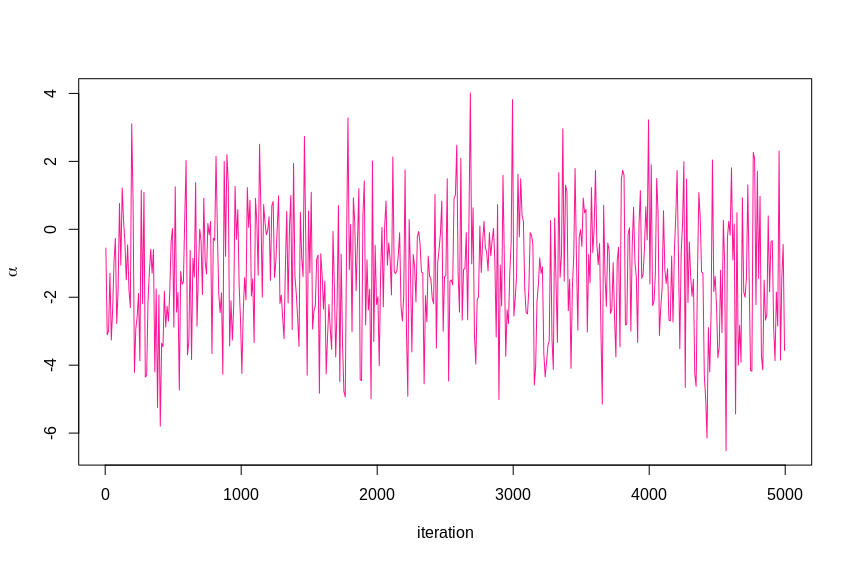
\includegraphics[width=0.8\linewidth]{img/esercizio10-2-1}% "%" necessario
    \qquad\qquad
    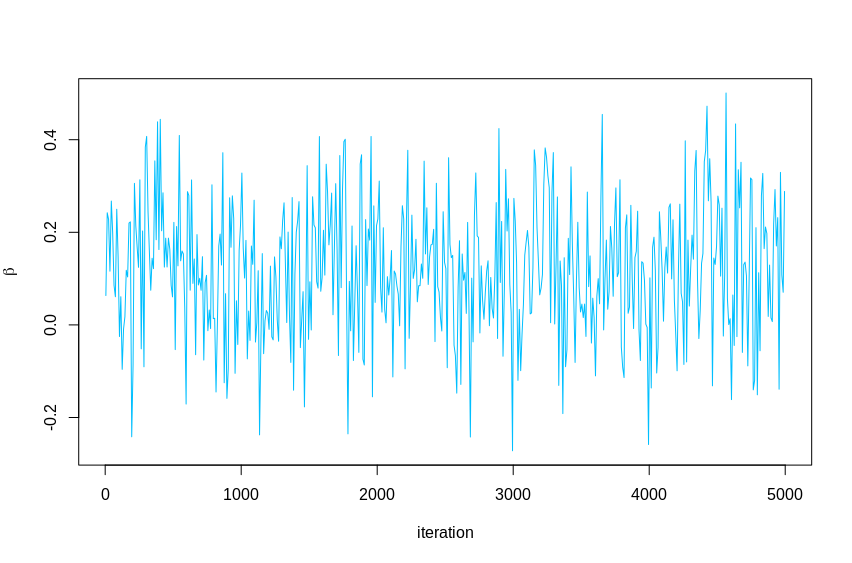
\includegraphics[width=0.8\linewidth]{img/esercizio10-2-2}
    \caption{}
  \end{figure}
  
  Facciamo adesso il confronto delle distribuzioni a priori e posteriori dei coefficienti di regressione:
  
  \begin{lstlisting}
  par(mfrow=c(1,2))
  x<-seq(-10, 10, by=0.1)
  plot(x, dnorm(x, pmn.beta[1], psd.beta[1]) ,ylim=c(0,0.25), type="l",lwd=1, xlab=expression(alpha), ylab="density", col = "orange")
  lines(density(beta.post[ ,1]) , col = "red")
  legend("topright",legend=c("Prior","Posterior"),lty = c(1,1),cex=0.7, bty="n",seg.len=1.5,  col = c("orange","red"))
  y<-seq(-2,2,by=0.01)
  plot(y,dnorm(y,pmn.beta[2],psd.beta[2]), ylim=c(0,3), type="l", lwd=1, xlab=expression(beta), ylab="density", col = "orange")
  lines(density(beta.post[ ,2]) , col="red")
  legend("topright",legend=c("Prior","Posterior"),lty = c(1,1),cex=0.7,bty="n", seg.len=1.5, col = c("orange","red"))
  \end{lstlisting}
  \begin{figure}[h!]
    \centering
    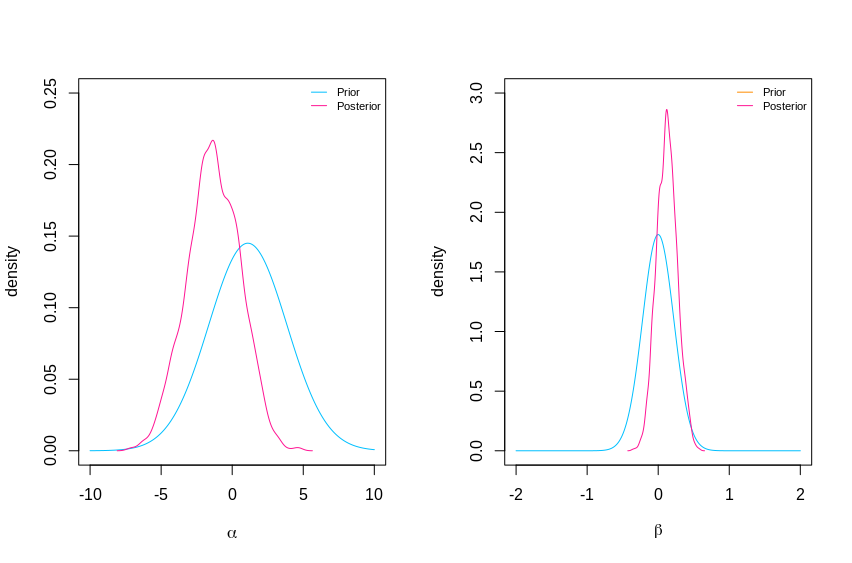
\includegraphics[width=0.7\linewidth]{img/esercizio10-2-3}
    \caption{}
    \label{fig:metropolis3}
  \end{figure}
  
  \begin{lstlisting}
    f<-exp(t(X%*%t(beta.post)))/(1+exp(t(X%*%t(beta.post))))
    qE<-apply(f,2,quantile,probs=c(0.025,0.975))
    par(mfrow=c(1,1))
    plot(c(10,15),range(c(0,qE)),type="n",xlab="wingspan",ylab="f")
    lines(qE[1,],col="deepskyblue",lwd=2)
    lines(qE[2,],col="deeppink",lwd=2)
  \end{lstlisting}

  Notiamo che la distribuzione a posteriori dà probabilità maggiore a valori più bassi di $\alpha$ e a valori più alti di $\beta$ rispetto a quella a priori. Questo significa che avevamo ipotizzato una proabilità di nidificare un po' troppo alta.\\
  
  Approssimiamo adesso la funzione richiesta nel punto e, utilizzando i risultati dell'algoritmo di Metropolis. Tracciamo anche la banda di confidenza al $95\%$.
  \begin{figure}[h!]
    \centering
    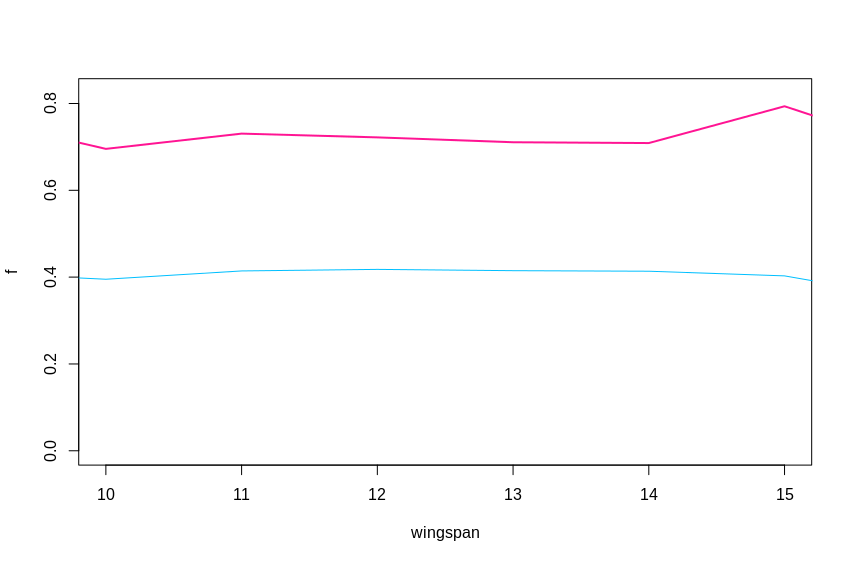
\includegraphics[width=0.7\linewidth]{img/esercizio10-2-4}
    \caption{}
    \label{fig:metropolis4}
  \end{figure}
  
  Dal grafico si evince che l'ampiezza delle ali non influenza la probabilità di nidificare poichè la banda di confidenza è praticamente parallela all'asse delle ascisse.
  
  
% \newpage
\subsubsection*{Esercizio 11.2 pag. 246 Hoff}

Randomized block design: researchers interested in identifying the optimal planting density for
a type of perennial grass performed the following randomized experiment: ten different plots of
land were each divided into eight subplots, and planting densities of 2, 4, 6 and 8 plants per
square meter were randomly assigned to the subplots, so that there are two subplots at each
density in each plot. At the end of the growing season the amount of plant matter yield was
recorded in metric tons per hectare. These data appear in the file pdensity.dat. The researchers
want to fit a model like $y = \beta_1 + \beta_2 x + \beta_3 x^2 + \epsilon$, where $y$ is yield and $x$ is planting density,
but worry that since soil conditions vary across plots they should allow for some across-plot
heterogeneity in this relationship. To accommodate this possibility we will analyze these data
using the hierarchical linear model described in Section 11.1.

\begin{enumerate}
    \item Before we do a Bayesian analysis we will get some ad hoc estimates of these parameters via
    least squares regression. Fit the model $y = \beta_1 +\beta_2 x+\beta_3 x^2 + \epsilon$ using OLS for each group,
    and make a plot showing the heterogeneity of the least squares regression lines. 
    From the least squares coefficients find ad hoc estimates of $\theta$  and $\Sigma$. 
    Also obtain an estimate of $\sigma$ 2 by combining the information from the residuals across the groups.
    \item Now we will perform an analysis of the data using the following distributions as prior distributions:
    $$ \Sigma^{-1} \sim \text{Wishart}(4, \hat\Sigma^{-1})$$
    $$ \theta \sim \text{multivariate normal} (\hat\theta, \hat\Sigma)$$
    $$ \sigma^2 \sim \text{inverse-gamma}(1, \hat\sigma^2)$$

    where $\hat\theta,|\hat\Sigma, \sigma^2 $ are the estimates you obtained in a). 
    Note that this analysis is not combining prior information with information from the data, as the “prior” distribution is based on
    the observed data. 
    However, such an analysis can be roughly interpreted as the Bayesian
    analysis of an individual who has weak but unbiased prior information.
    
    \item Use a Gibbs sampler to approximate posterior expectations of $\beta$ for each group $j$, and plot
    the resulting regression lines. Compare to the regression lines in a) above and describe why
    you see any differences between the two sets of regression lines.

    \item From your posterior samples, plot marginal posterior and prior densities of $\theta$ and the
    elements of $\Sigma$. 
    Discuss the evidence that the slopes or intercepts vary across groups.
    \item Suppose we want to identify the planting density that maximizes average yield over a
    random sample of plots. 
    Find the value $x_max$ of x that maximizes expected yield, and
    provide a 95\% posterior predictive interval for the yield of a randomly sampled plot having
    planting density $x_max$.
\end{enumerate}

\subsubsection*{Premessa e indicazioni generali}
Si vuole valutare la relazione tra raccolto e densità di piante
relativamente a 10 lotti di terra osservati nel seguente modo:

\begin{itemize}[-]
    \item 10 lotti di terra.
    \item Un lotto comprende altri 8 sottolotti.
    \item Densità di piantagione pari a 2, 4, 6 e 8 sono assegnate in maniera casuale tra
    gli 8 sottolotti in modo tale che ogni lotto ha due sottolotti di ognuna delle densità.
\end{itemize}

È richiesta l'analisi della relazione tra raccolto e densità mediante un modello di regressione
lineare quadratica e tenendo conto della variabilità tra gruppi in termini di condizioni di suolo.
Per come è costruito il disegno e per come è formulato il modello procediamo nel'analisi attraverso
un modello di regressione lineare gerarchico. Il setting del modello è:\\

\begin{itemize}[-]
	\item $ Y_{ij} = {\beta^T_jx_{ij}} + \varepsilon_{ij}$;
	\item $\varepsilon_{ij}|\sigma^2 \sim i.i.d. N(0,\sigma^2)$.
\end{itemize}

cioè:

\begin{itemize}[-]
	\item $Y_j | \beta_j, X_j, \sigma^2 \sim N_{n_j} ({X_j \beta_j}, \sigma^2 {I})$\quad
	$i = 1, \dots, n;\ \  j = 1, \dots, m$; 
	\item $ \beta_j | \theta, \Sigma \stackrel{iid}{\sim} N_{p} (\theta, \Sigma)$;
	\item $\theta| \mu_0,\Lambda_0 \sim N_p(\mu_0,\Lambda_0) $;
	\item $\Sigma \sim \text{\normalfont{Inverse - Wishart}}(\eta_0, S_0{-1})$;
	\item $ \sigma^2 | v_0, \sigma^2_0\sim \text{\normalfont{Inverse - Gamma}}(\frac{v_0}{2}, \frac{v_0\sigma^2_0}{2})$;
	\item $ Y_i \perp Y_j | \beta_1, \dots, \beta_m, \sigma^2 i \neq j$.
\end{itemize}

In seguito si riporta il codice R.

\begin{lstlisting}[style=R]
#Funzione per campionare da una normale multivariata:
rmvnorm<-
function(n,mu, Sigma ) {
    p<-length(mu)
    res<-matrix ( 0, nrow=n, ncol=p)
    if ( n>0 & p>0 ) {
        E<-matrix( rnorm(n*p),n, p)
        res<-t ( t (E%*%chol ( Sigma ) ) +c (mu) )
        #R <- chol(A)
}
res
}

#Funzione per campionare da una Wishart:
rwish<-function (n, nu0, S0 )
{
    sS0 <- chol( S0 )
    S<-array ( dim=c ( dim( S0 ),n ) )
    for ( i in 1: n)
    {
        Z <-matrix ( rnorm( nu0 * dim( S0 ) [ 1 ] ), nu0, dim( S0 ) [ 1 ] ) %*% sS0
        + S [,, i ]<-t (Z)%*%Z
    }
    S [,, 1: n ]
}

#Funzione per campionare da una Inverse-Wishart:

rinvwish<-function(n, nu0, iS0 )
{
    sL0 <- cho l ( iS0 )
    S<-array ( dim=c ( dim( iS0 ),n ) )
    for ( i in 1: n)
{
    Z <- matrix ( rnorm( nu0 * dim( iS0 ) [ 1 ] ), nu0, dim( iS0 ) [ 1 ] ) %*% sL0
    S [,, i ]<- solve ( t (Z)%*%Z)
}
    S [,, 1: n ]
}

#Lettura dei dati:

dati<-read.table("C:\\Desktop\\pdensity.dat", header=TRUE)



\end{lstlisting}
{
\color{red}
\begin{Verbatim}
> head (dati)

plot density yield
1       2     8.25
1       2     5.81
1       4     8.69
1       4     8.03
1       6     7.96
1       6     8.89
\end{Verbatim}
}

\begin{lstlisting}[style=R]
#Calcolo di quantita' utili per ogni gruppo ( numerosita', vettore delle osservazioni, matrice del modello e numero di parametri ):
ids<-unique (datis$plot )
m<-length ( ids )
Y<-list() ; X<-list() ; N<-NULL
for ( j in 1:m)
{
    Y[ [ j ]]<-dati [ dati [,1]== ids [ j ], 3]
    N[ j]<- sum( dati$plot==ids [ j ])
    xj<-dati [ dati [,1]== ids [ j ], 2]
    X[ [ j ]]<-cbind ( rep (1,N[ j ]), xj, xj^2 )
}
p<-dim(X[ [ 1 ] ] ) [2]

\end{lstlisting}

{
\color{red}
\begin{verbatim}
> N

[1] 8 8 8 8 8 8 8 8 8 8
\end{verbatim}
}

{
\color{red}
\begin{verbatim}
> Y[ [ 1 ] ]

[1] 8.25 5.81 8.69 8.03 7.96 8.89 6.13 9.40    
\end{verbatim}
}

{
\color{red}
\begin{verbatim}
> X[ [ 1 ] ]

     xj
[1,] 1 2 4
[2,] 1 2 4
[3,] 1 4 16
[4,] 1 4 16
[5,] 1 6 36
[6,] 1 6 36
[7,] 1 8 64
[8,] 1 8 64
\end{verbatim}
}

\subsubsection*{Punto a)}
\begin{lstlisting}[style=R]
#Stimiamo i coefficienti di regressione secondo il metodo OLS
#indipendentemente in ciascuno de i 10 lotti:
S2.OLS<-BETA.OLS<-NULL
for( j in 1:m) {
    fit<-lm(Y[ [ j ]]~-1+X[ [ j ] ] )
    BETA.OLS<-rbind (BETA.OLS, c ( fit$coef ) )
    S2.OLS<-c ( S2.OLS, summary( fit )$sigma ^2)
}

colnames (BETA.OLS)<-c ("1"," x "," x^2")
\end{lstlisting}

{
\color{red}
\begin{Verbatim}
> BETA.OLS

            1       x         x^2
[1,]    4.84000 1.357250 -0.1243750
[2,]    4.53375 1.193375 -0.1290625
[3,]    2.07750 2.128250 -0.1643750
[4,]    2.60375 2.114875 -0.1928125
[5,]    3.57000 1.540500 -0.1500000
[6,]    1.47375 1.930875 -0.1215625
[7,]    3.96375 1.424875 -0.1278125
[8,]    0.52375 2.941875 -0.2653125
[9,]    3.36250 1.675500 -0.1400000
[10,]   1.73875 2.241125 -0.1771875
\end{Verbatim}
}

{
\color{red}
\begin{Verbatim}
> S2.OLS

[1] 1.8005320 1.0760545 0.8134580 0.5019505 0.5886680 0.8074545 0.9575905
[8] 0.3965025 0.1328380 0.8030505
\end{Verbatim}
}

\begin{lstlisting}[style=R]
# Rappresentiamo graficamente le 10 linee di regressione per valutare la variabilita' tra gruppi. 
# Riportiamo sul grafico anche la loro media.

par (mfrow=c (1,2) )
plot ( range ( dati [,2]), range ( dati [,3]), type="n", xlab="planting density ", +ylab="Expected yield ",main="Regression lines OLS")
for ( j in 1:m) {curve (BETA.OLS[ j,1]+BETA.OLS[ j,2]* x+BETA.OLS[ j,3]* x^2,
col="gray ",add=T)}
BETA.OLS.MEAN<-apply (BETA.OLS,2,mean)
curve (BETA.OLS.MEAN[1]+BETA.OLS.MEAN[2]* x+BETA.OLS.MEAN[3]* x^2,lwd=2,add=T)

\end{lstlisting}

\begin{figure}
    \centering
    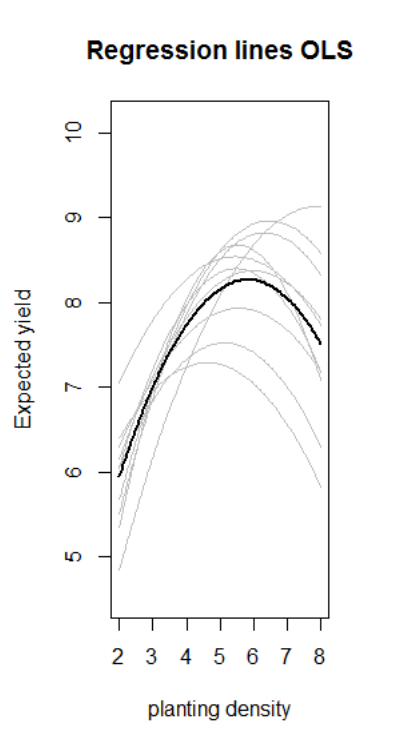
\includegraphics[totalheight=8cm]{img/esercizio11-2-1.png}
    \caption{ Curve di regressione con stime OLS.}
\end{figure}

{
\color{red}
\begin{Verbatim}
> BETA.OLS.MEAN

    1       x       x^2
2.86875 1.85485 -0.15925
\end{Verbatim}
}

{
\color{red}
\begin{Verbatim}
> cov(BETA.OLS)

        1           x           x^2
1 2.00120764    -0.69321313  0.044309549
x -0.69321313    0.27555421 -0.020742679
x 2 0.04430955  -0.02074268  0.001968451
\end{Verbatim}
}

{
\color{red}
\begin{Verbatim}
> mean(S2.OLS)

[1] 0.7878099
\end{Verbatim}
}

Si osserva che:
\begin{itemize}
    \item Tutte le curve hanno lo stesso andamento quadratico: crescente fino ad una densità di piante pari circa a 6 e poi decrescente.
    \item Alcuni gruppi si discostano particolarmente dalla media generale: il raccolto medio risulta o molto inferiore o molto superiore, soprattutto per i valori più grandi del range della covariata. Nel caso in cui i lotti avessero diverse numerosità al loro interno potremmo immaginare che questo si verifica per i lotti meno numerosi ; in realtà per come è disegnato l' esperimento questa variabilità osservata è dovuta ad altro, forse alle diverse condizioni del terreno dei 10 appezzamenti.
\end{itemize}

\subsubsection*{Punto b)}
\begin{lstlisting}[style=R]
#Setting delle prior: impostiamo le prior semiconiugate per theta, Sigma e sigma2 come richiesto. Ricordiamo che le prior sono specificate in ottica empirico-bayesiana e che quindi l' analisi non combina le informazioni a priori con quelle a posteriori ma puo' essere all' incirca interpretata come quella di un individuo con informazione debole, ma non distorta.
theta<-BETA.OLS.MEAN; Sigma<-cov(BETA.OLS) ; sigma2<-mean(S2.OLS)
eta0 <-4; S0<-Sigma
mu0<-theta ; L0<-Sigma
v0<-2; sigma20<-sigma2
\end{lstlisting}

\subsubsection*{Punto c)}
Impostiamo come richiesto un Gibbs sampler: infatti è possibile approssimare in questo modo la distribuzione a posteriori dal momento che usiamo prior semiconiugate. 
Per le distribuzioni full conditional si veda il quaderno.

\begin{lstlisting}[style=R]
#Numero di simulazioni:

nsimul=10000

#Valori iniziali dei parametri:

beta<-BETA.OLS
Sigma<-cov(BETA.OLS)
sigma2<-mean(S2.OLS)

#Oggetti in cui inseriamo durante l' algoritmo i valori campionati dalle full conditional:

Sigma.post<-matrix (0,p,p)
BETA.pp<-THETA.POST<-S2.POST<-NULL
BETA.POST<-BETA.OLS*0
SIGMA.POST<-array (0, c(p,p, nsimul ) )
set.seed (1)

#Algoritmo Gibbs per nsimul iterazioni
for ( s in 1: nsimul ) {
    for ( j in 1:m)
    {
        #Per ogni gruppo campioniamo i coefficienti di regressione:

        Vj<-solve ( solve (Sigma) + t (X[ [ j ] ] )%*%X[ [ j ]]/ sigma2 )
        Ej<-Vj%*%( solve (Sigma)%*%theta + t (X[ [ j ] ] )%*%Y[ [ j ]]/ sigma2 )
        beta [ j,]<-rmvnorm(1,Ej, Vj)
    }

    #Campioniamo la supermedia theta dei coefficienti di regressione:
    Lm<- solve ( solve (L0) + m* solve (Sigma) )
    mum<- Lm%*%( solve (L0)%*%mu0 + solve (Sigma)%*%apply ( beta,2,sum) )
    theta<-t (rmvnorm(1,mum,Lm) )

    #Campioniamo la matrice di varianza e covarianza Sigma dei coefficienti di regressione:
    mtheta<-matrix ( theta,m,p, byrow=TRUE)
    Sigma<-solve ( rwish (1, eta0+m, solve ( S0+t ( beta-mtheta)%*%(beta-mtheta) ) ) )
    #Campioniamo la varianza residua:

    RSS<-0
    for ( j in 1:m) { RSS<-RSS+sum( (Y[ [ j ]]-X[ [ j ]]%*%beta [ j, ] )^2 ) }
    sigma2<-1/rgamma(1,( v0+sum(N) ) /2, (v0*sigma20+RSS)/2 )
    #Immagazziziniamo i valori appena campionati:
    S2.POST<-c(S2.POST, sigma2 ) ;THETA.POST<-rbind (THETA.POST, t ( theta ) )
    Sigma.post<-Sigma.post+Sigma ; BETA.POST<-BETA.POST+beta
    SIGMA.POST[,, s]<-Sigma
    #Campioniamo dalla posterior predictive dei coefficienti di regressione che ci servira' per il punto e).
    BETA.pp<-rbind (BETA.pp,rmvnorm(1, theta, Sigma) )
}
colnames (THETA.POST)<-c(" theta1 "," theta2 "," theta3 ")
colnames (BETA.POST)<-colnames (BETA. pp)<-c(" beta1 "," beta2 "," beta3 ")

#Plottiamo adesso le curve di regressione con le stime dei coefficienti derivanti dal Gibbs sampler per poi confrontarle con quelle precedenti in caso di stima OLS. Anche in questo caso la media delle curve e' di colore nero.

BETA.PM<-BETA.POST/nsimul
plot ( range (c (0,10) ), range (c (0,10) ), type="n",
xlab="planting density ", ylab="Yield ",main="Bayesian regression lines ")
for ( j in 1:m) { curve (BETA.PM[ j,1]+BETA.PM[ j,2]* x+BETA.PM[ j,3]* x^2,
col="gray ",add=T)}
curve ( mean(THETA.POST[,1])+mean(THETA.POST[,2]) *x+
mean(THETA.POST[,3]) *x^2,lwd=2,add=T )
#dev.off ()

#Controlliamo la convergenza dell' algoritmo:

library (coda)

\end{lstlisting}
Osservando i due grafici a confronto si nota che il modello gerarchico permette 
di trarre informazioni dai gruppi, 
riportando le curve di regressione lungo la media. 
In particolare vediamo adesso che l'andamento delle curve è ancora più simile 
rispetto al caso OLS e che per valori più grandi del range di x il valore 
atteso del raccolto è sì sempre più basso in alcuni casi e sempre più alto in 
altri rispetto alla media, ma con un'intensità minore. 
Dal momento che lavoriamo con gruppi tutti di piccola numerosità c'è una grande 
variabilità nelle stime OLS mentre nel caso del modello gerarchico i gruppi si 
influenzano in termini di informazioni e per l'effetto di shrinkage la stima OLS 
viene portata verso la stima media in modo uguale per tutti i gruppi perché hanno 
la stessa numerosità campionaria.
\begin{figure}
    \centering
    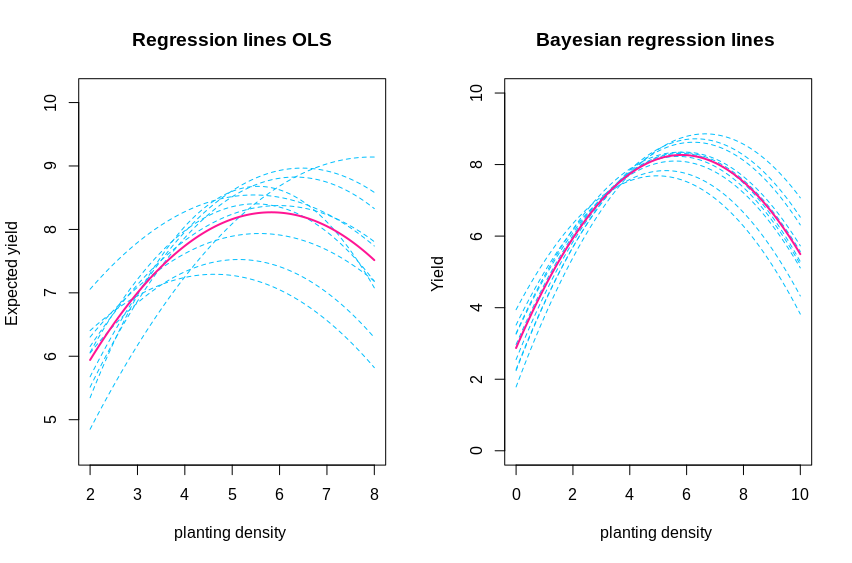
\includegraphics[totalheight=8cm]{img/esercizio11-2-2.png}
    \caption{ GLMM: stime dei minimi quadrati e stime bayesiane a confronto.}
\end{figure}
\newpage
{
\color{red}
\begin{Verbatim}
> effectiveSize (THETA.POST)

theta1   theta2   theta3  
6938.395 7144.829 7501.045 
\end{Verbatim}
}

\subsubsection*{Punto d)}
\begin{lstlisting}[style=R]
#Approssimazione delle distribuzioni a priori tramite simulazione Monte Carlo ( facciamo notare che potremmo derivarle anche analiticamente ):

n<-10000

THETA.PRIOR<-rmvnorm(n,mu0,L0) ; colnames (THETA.PRIOR)<-colnames (THETA.POST)
SIGMA.PRIOR<-rinv
\end{lstlisting}

\newpage
{
\color{red}
\begin{Verbatim}
> head(THETA.PRIOR)

           theta1      theta2     theta3
[1,]  -1.77780314    3.529232 -0.2613000
[2,]   3.47065885    1.752018 -0.1395134
[3,]   3.60717709    1.583506 -0.1350985
[4,]   0.07323521    2.928965 -0.2604753
[5,]   3.05388848    1.832459 -0.1571405
[6,]   2.27382048    1.786574 -0.1183835
\end{Verbatim}
}

{
\color{red}
\begin{Verbatim}
> head(SIGMA.PRIOR)

[1] 3.63026418 -0.93710237 0.04650011 -0.93710237 0.28263581 -0.01833983
\end{Verbatim}
}

\begin{lstlisting}[style=R]
#A priori e a posteriori di theta a confronto ( plot ):

par (mfrow=c (2,2) )
for ( i in 1:3) {
    plot ( density (THETA.POST[, i ]), xlab=paste (" theta ", i ),main="")
    lines ( density (THETA.PRIOR[, i ]), col="grey ")
    legend (" topright ", legend=c(" Prior "," Posterior "), col=c(" grey "," black "),
    lty =1,bty="n", cex =0.7)
}
\end{lstlisting}

\begin{figure}
    \centering
    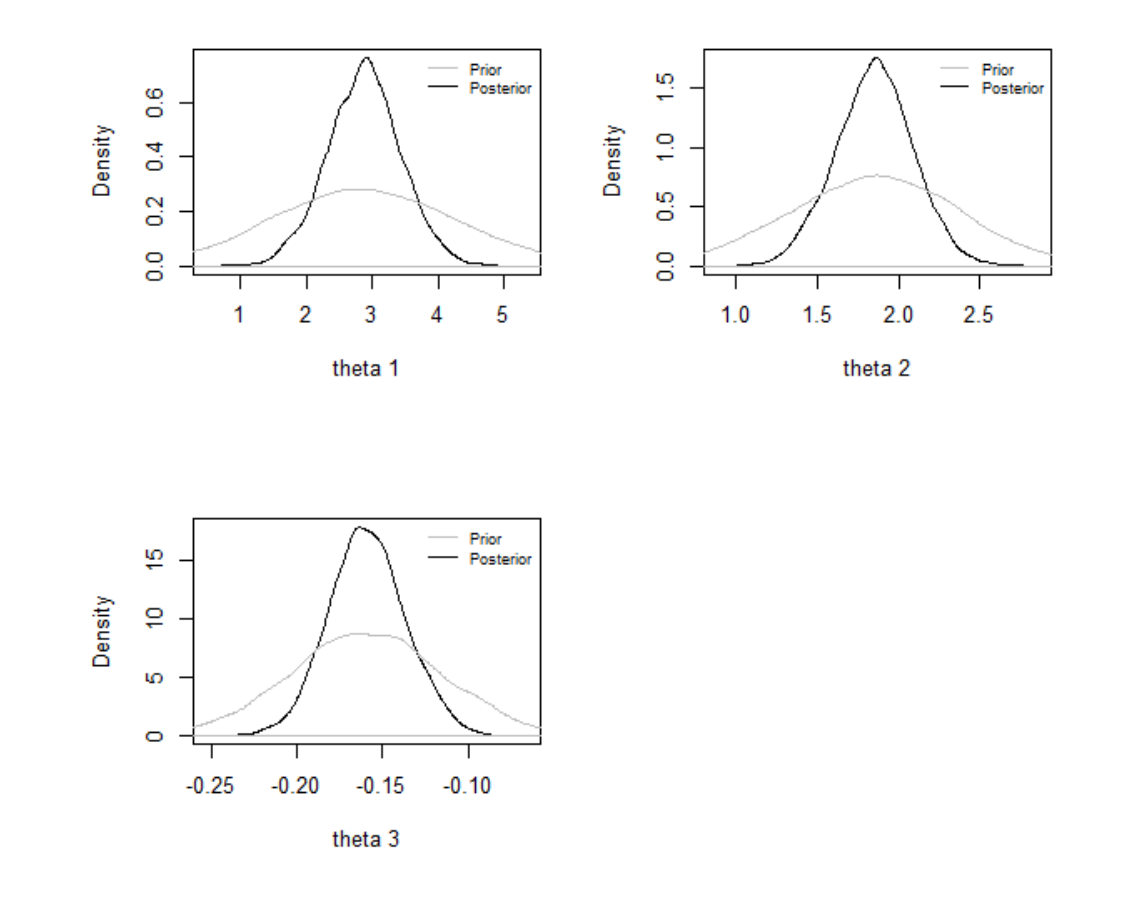
\includegraphics[totalheight=8.5cm]{img/esercizio11-2-3.png}
    \caption{  Densità a priori e a posteriori a confronto (media).}
\end{figure}

Si osserva che le distribuzioni a posteriori, pur essendo centrate sulla stessa 
media delle a priori (come ci aspettavamo dal momento che abbiamo centrato le 
prior nelle stime di massima verosimiglianza ), sono meno diffuse: 
in questo modo l'informazione a posteriori cambia nel senso che si dà maggiore 
probabilità ai valori che cadono attorno ad essi.

\begin{lstlisting}[style=R]
#Prior e posterior di Sigma a confronto ( plot ):

par (mfrow=c (2,2) )
for ( i in 1:3) {
plot ( density ( log (SIGMA.POST[ i, i, ] ) ), type="l ", xlab=paste ("Sigma", i ),
ylab="density ",main="")
lines ( density ( log (SIGMA.PRIOR[ i, i, ] ) ), col="gray ",lwd=2)
legend (" topright ", legend=c(" Prior "," Posterior "), col=c(" gray "," black "),
bty="n", lty=1)
}
\end{lstlisting}

N.B. Abbiamo preso il logaritmo degli elementi di Sigma dal momento che sono valori 
molto bassi. N.B. Dal momento che è richiesto di commentare la variabilita' 
relativa all' intercetta e alle pendenze nei gruppi, 
riportiamo i plot delle distribuzioni dei soli elementi della diagonale principale di 
Sigma. 

Commento al plot: è evidenza che la variabilità tra i gruppi delle intercette non è 
molto elevata, ma diminuisce ancora per il primo e per il secondo coefficiente 
(ricordiamo che dal momento che consideriamo il logaritmo delle varianze la 
variabilità è minore è indicata da una densità concentrata su valori sempre più 
negativi.


\subsubsection*{Punto e)}
Si vuole trovare la densità di piante che massimizza il raccolto atteso 
per un campione di lotti. Ricordiamo che stiamo lavorando con un modello 
gerarchico e quindi vogliamo tenere in considerazione anche la variabilità tra gruppi: 
ci serviamo a questo scopo della distribuzione predittiva a posteriori dei 
coefficienti di regressione (una normale multivariata con vettore delle medie e 
matrice di varianza e covarianza pari quelli estratti ad ogni passo dell'algoritmo ) 
per cui ogni vettore di coefficienti estratto rappresenta il vettore dei coefficienti 
di regressione per un gruppo futuro. Disponiamo già di tale distribuzione dal 
momento che è stata calcolata durante l'algoritmo. 
Necessario adesso confrontare 4 distribuzioni: quelle dei valori attesi del 
raccolto di un generico lotto, una per ogni valore osservato della covariata x. 
Anche in questo caso vogliamo tenere in considerazione la variabilità tra lotti e per 
questo approssimiamo le distribuzioni usando la predittiva a posteriori dei 
coefficienti di regressione appena discussa. Cerchiamo il valore atteso di y date 
le y passate e le x. Un modo per farlo è campionare i beta dalla loro posterior 
predictive e capionare le y dati i valori della x e quindi per ogni valore della x 
potevamo avere un valore atteso. Facciamo la media delle distribuzioni dei valori 
attesi. Campioniamo i beta tilde: i beta per un gruppo futuro. Per ogni valore di 
questo beta campinato abbiamo un valore del valore atteso per un y futuro. 
Alla fine per ogni x si genera una distribuzione del valore atteso della y futuro 
(4 vettori ). Confrontiamo le 4 distribuzioni ( per es con la media o vedendo la 
prob. che una sia maggiore dell'altra ). Prendendo il valore medio per ogni valore 
di beta tilde e per l' ixmax e la varianza a posteriori campiono un valore y. 
Così si incorpora anche l'incertezza derivante dai gruppi.

\begin{lstlisting}[style=R]
x0<-c (2,4,6,8)
raccolto<-NULL
for ( i in x0){
x<-c (1, i, i ^2)
raccolto<-cbind ( raccolto,BETA. pp%*%x)
}
colnames ( raccolto )<-x0
\end{lstlisting}


\begin{figure}
    \centering
    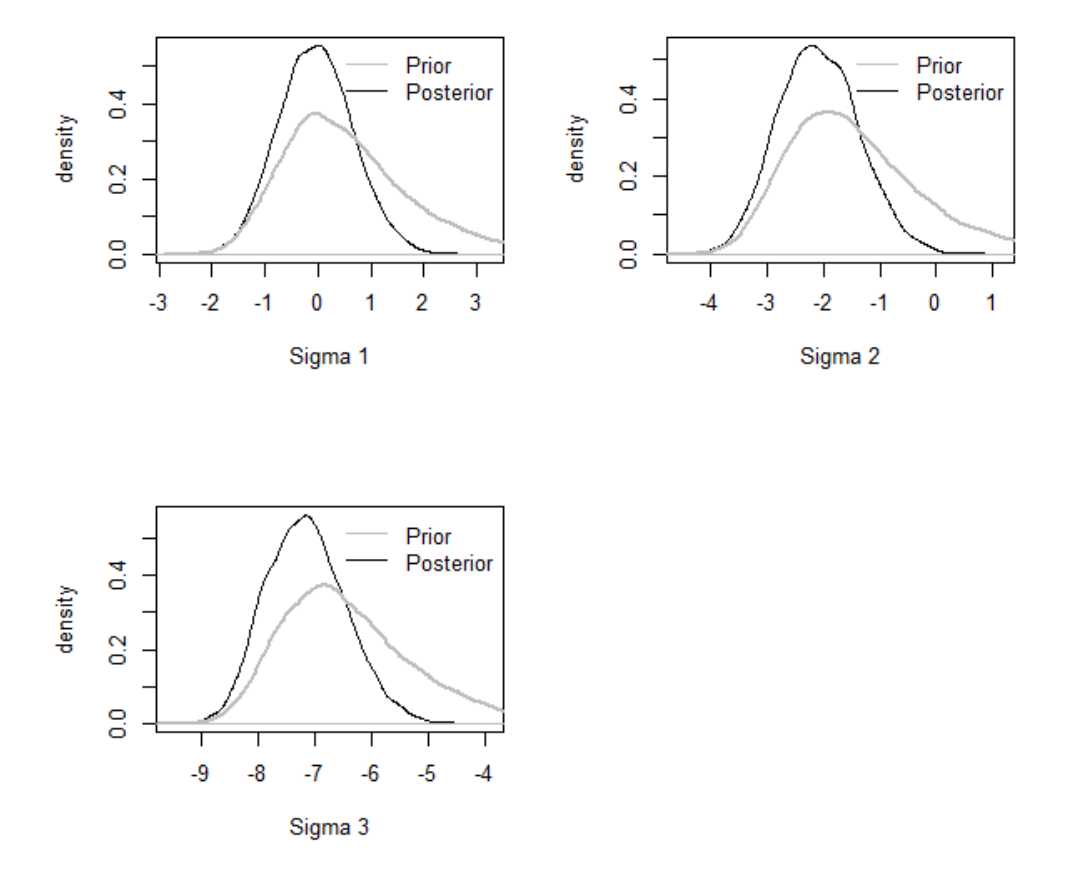
\includegraphics[totalheight=10cm]{img/esercizio11-2-4.png}
    \caption{  Densità a priori e a posteriori a confronto (variabilità e covariabilità).}
\end{figure}

{
\color{red}
\begin{Verbatim}
> head( raccolto )

            2        4        6        8
[1,] 5.989406 7.758386 8.317531 7.666840
[2,] 6.033526 7.921516 8.605911 8.086712
[3,] 6.350655 7.597301 7.712147 6.695192
[4,] 6.888414 7.776763 7.907158 7.279599
[5,] 5.973396 7.669427 8.482208 8.411740
[6,] 6.247427 7.685203 7.955526 7.058398
\end{Verbatim}
}

\begin{lstlisting}[style=R]
#Confrontiamo adesso le quattro distribuzioni dei valori attesi,
#graficamente e con un indice sintetico, la media:

par (mfrow=c (1,1) )
hist ( raccolto [,1], prob=T, main="Raccolto atteso a posteriori ", xlab="Raccolto ",
xlim=c (2,13), ylim=c (0,1.5) )
lines ( density ( raccolto [,1]) )
hist ( raccolto [,2], prob=T, col="red ",add=T)
lines ( density ( raccolto [,2]), col="red ")
hist ( raccolto [,3], prob=T, col="green ",add=T)
lines ( density ( raccolto [,3]), col="green ")
hist ( raccolto [,4], prob=T, col="blue ",add=T)
lines ( density ( raccolto [,4]), col="blue ")
legend (" topright ", legend=c("x=2","x=4","x=6","x=8"), col=c(" black "," red ",
"green "," blue "), lty=1)
\end{lstlisting}

{
\color{red}
\begin{Verbatim}
> apply ( raccolto,2,mean)
       2        4        6        8
5.942984 7.739188 8.264142 7.517844
\end{Verbatim}
}

\begin{figure}
    \centering
    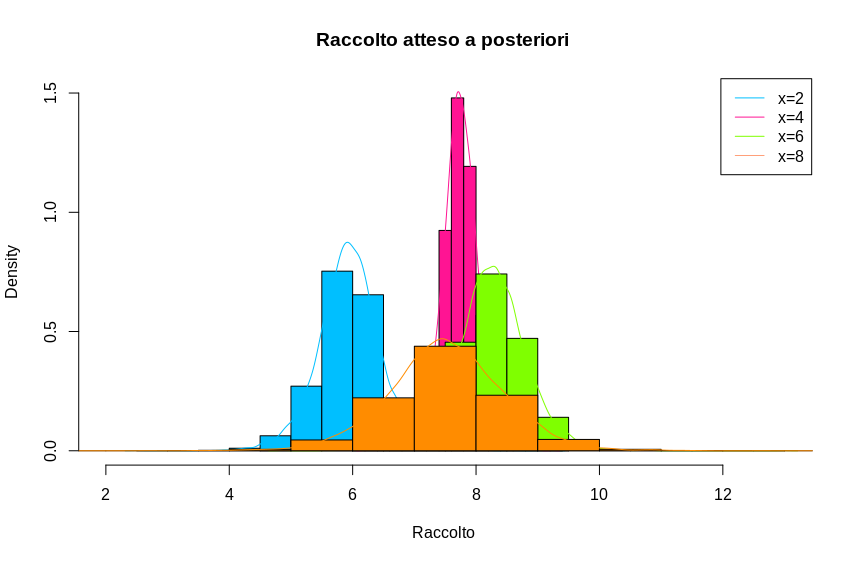
\includegraphics[totalheight=8cm]{img/esercizio11-2-5.png}
    \caption{  Valori attesi a posteriori per più valori di x a confronto.}
\end{figure}

Si osserva che il valore della covariata che masimizza il raccolto atteso per un 
generico lotto è x=6. Procediamo quindi considerando tale valore per il predittore 
lineare. Si vuole infine approssimare la distribuzione predittiva a posteriori per 
un generico lotto avendo una densità di piantagioni pari a 6. La logica è la stessa 
di quella usata per la predittiva a posteriori dei coefficienti di regressione, con 
la differenza che adesso siamo al livello più basso della gerarchia e quindi si 
aggiunge un parte di variabilità dovuta alle osservazioni campionarie. 
Per ogni vettore dei coefficienti estratto dalla predittiva a posteriori e per ogni 
elemento estratto dalla a posteriori della varianza residua ( anche questo fatto già 
fatto nell' algoritmo ) campioniamo un valore del raccolto da una normale con 
media pari al predittore lineare e varianza pari alla varianza residua. 
Riportiamo infine un plot della densità e l' intervallo di confidenza richiesto per 
tale distribuzione:

\begin{lstlisting}[style=R]
y.pred<-rnorm( nsimul,BETA.pp%*%x, S2.POST)
\end{lstlisting}

{
\color{red}
\begin{Verbatim}
> quantile (y.pred, c (0.025,0.975) 

    2.5%    97.5%
5.213170 9.855576
\end{Verbatim}
}

\begin{lstlisting}[style=R]
hist(y. pred, prob=T, main="Predittiva a posteriori ", xlab="raccolto ")
lines (y. pred )
\end{lstlisting}

\begin{figure}
    \centering
    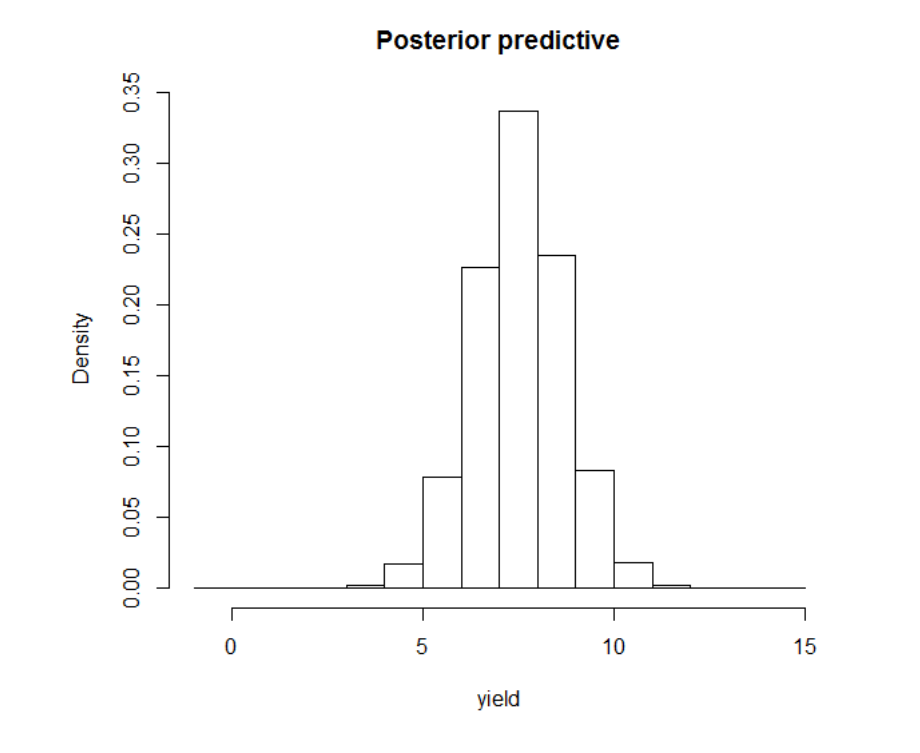
\includegraphics[totalheight=10cm]{img/esercizio11-2-6.png}
    \caption{   Predittiva a posteriori.}
\end{figure}
	
\end{document}